%%%%%%%%%%%%%%%%%%%%%%%%%%%%%%%%%%%%%%%%%%%%%%%%%%%
%
%  New template code for TAMU Theses and Dissertations starting Fall 2016.  
%
%
%  Author: Sean Zachary Roberson
%  Version 3.17.09
%  Last Updated: 9/21/2017
%
%%%%%%%%%%%%%%%%%%%%%%%%%%%%%%%%%%%%%%%%%%%%%%%%%%%

%%%%%%%%%%%%%%%%%%%%%%%%%%%%%%%%%%%%%%%%%%%%%%%%%%%%%%%%%%%%%%%%%%%%%%%
%%%                           SECTION II
%%%%%%%%%%%%%%%%%%%%%%%%%%%%%%%%%%%%%%%%%%%%%%%%%%%%%%%%%%%%%%%%%%%%%%


\chapter{METHODS} 
\section{Basic Altimeter Test Bed Setup} \label{sec:Basic}
In addition to laying out performance standards for radar altimeters, the DO-155 standards~\cite{noauthor_minimum_1974} also specify a basic test setup for verifying an altimeter is functioning properly. Figure~\ref{fig:Basic Testbed} shows the diagram of this test setup, which connects the RF terminals of the altimeter to an \textit{altitude simulator} and connects a separate device to read altitude data.  
\begin{figure}[ht]
\centering
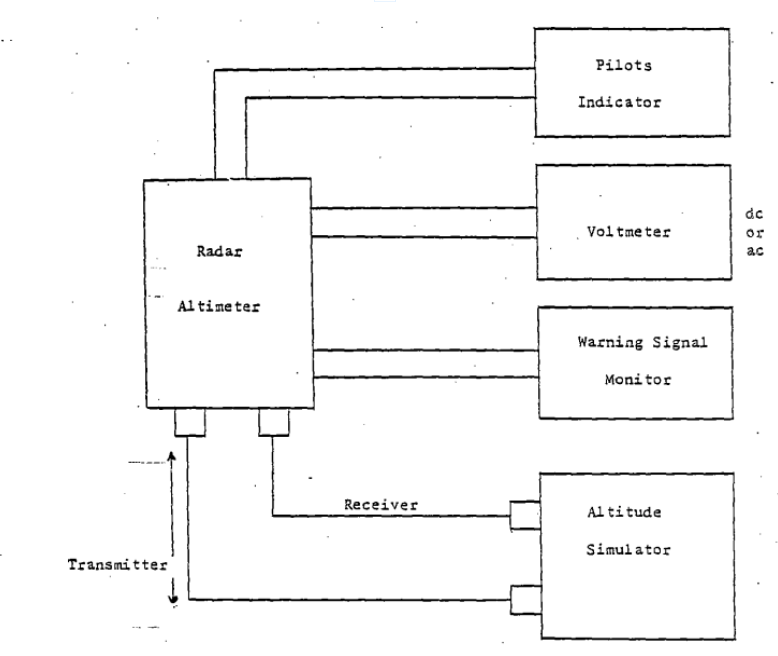
\includegraphics[scale=0.5]{DO-155_Test_Setup.PNG}
\caption{Basic Altimeter Test Setup from DO-155~\cite{noauthor_minimum_1974}}

\label{fig:Basic Testbed}

\end{figure}

The standards elaborated on the necessary characteristics of the most critical part of the test-bed, the altitude simulator. The altitude simulator needed to ``consist of variable and fixed RF attenuators''~\cite{noauthor_minimum_1974}  to simulate the loop loss an altimeter experiences aboard an aircraft (see section 1.6.3). The altitude simulator also needed a length of ``coaxial cables or other suitable delays''~\cite{noauthor_minimum_1974}  to simulate the physical time delay experienced by an altimeter signal between the transmitter and receiver (see Section~1.6.2). To complete the test setup, the altitude simulator directed the attenuated and delayed RF energy from the transmitter fed back into the receiver. 
%COMMENT: Use \ref for sections.


Additionally, the standards specified that any test equipment must account for cross coupling between transmitting and receiving antennas. The setup used for these tests would be verified by radar experts to adequately compensate for that. DO-155 emphasized that the altitude simulator should achieve the desired altitude within 1\% and the correct attenuation within 2.5~dB~\cite{noauthor_minimum_1974}. However, for the purposes of looking at the effects of interference, the absolute altitude is less important in these tests. 

%%%%%%%%%%%%%%%%%%%%%%%%%%%%%%%%%%%%%%%%%%%%%%%%%%%%%%%%%
\section{Modified Altimeter Test Setup} \label{sec:Modified}
\begin{figure}[ht]
\centering
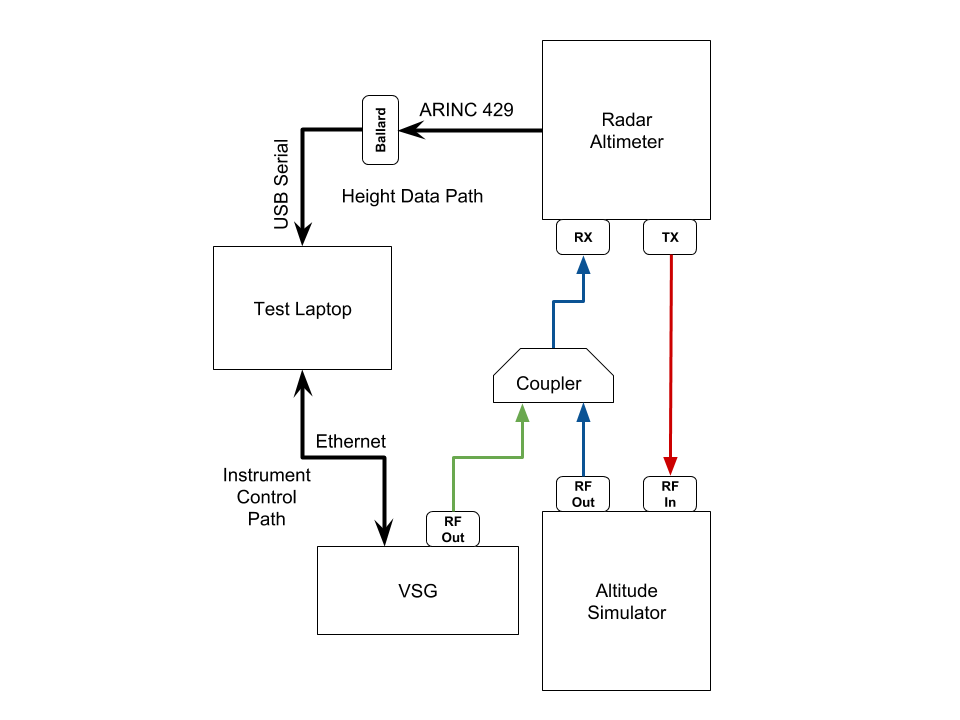
\includegraphics[scale=0.45]{Modified_Test_Setup.png}
\caption{Modified Altimeter Test Setup.}
% Comment: Make complete caption sentences.
\label{fig:Modified}

\end{figure}
AVSI designed a modified version of the altimeter test setup specified by DO-155, shown in Figure~\ref{fig:Modified}. The modifications allow the controlled injection of interference into the line after the altimeter signal passes  through the altitude simulator. 


\subsection{Reading the Altimeter Output}\label{sub:reading_out}
The altimeter outputs labeled height data on a standardized ARINC 429 cable configuration. The modified setup uses a Ballard ARINC device to convert the data from ARINC 429 to USB serial format, providing each data point with a time stamp. On the test laptop, Ballard CoPilot software reads the serial data and provides a display which allows the real time monitoring of all altimeter output and labels. 

The labels are critical because some data points may be labeled NCD (No Computed Data) when conditions are insufficient for a reliable height measurement. CoPilot software also allows for the easy export of test data to Microsoft Excel documents for post processing. 
\subsection{Implementing the Altitude Simulator}\label{sub:Implementing}

\begin{figure}[ht]
\centering
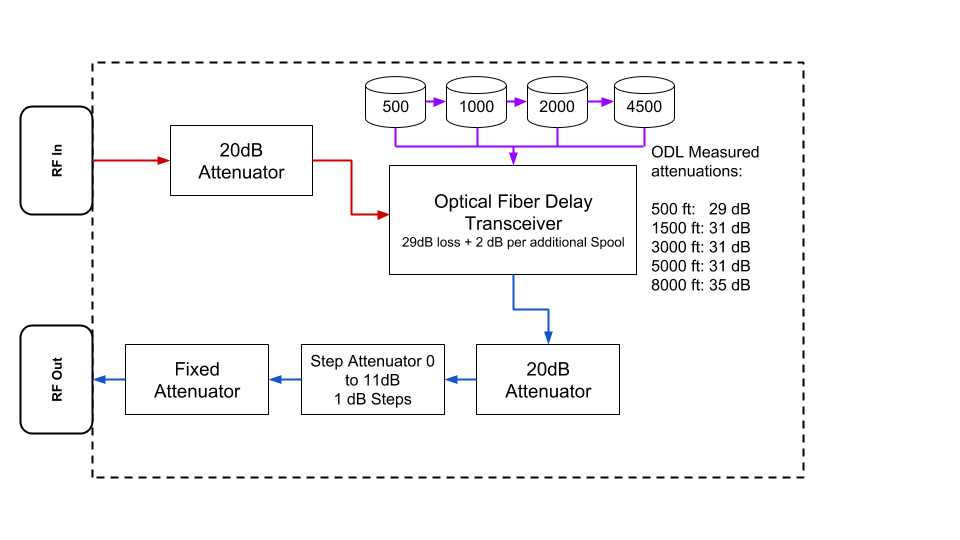
\includegraphics[width = 6 in]{Altitude_Simulator.png}
\caption{Internal Diagram of Altitude Simulator using optical delay line.}
% Comment: Make complete caption sentences.

\label{fig:Altitude_Simulator}

\end{figure}

\subsubsection{Time Delay}\label{subsub:delay}
Different test altitudes require the use of different methods of delaying the RF energy output by the altimeters. For the initial tests at higher altitudes, spools of fiber optic cables create a time delay as shown in Figure~\ref{fig:Altitude_Simulator}. The RF output from the altimeter transmitter was fed by coax connection to the fiber optic transceiver, which could either pass the signal to a single fiber optic spool or a series of cascaded spools to achieve a desired height. This setup contained optical spools of 500, 1000, 2000, and 4500 feet, each of which could be used individually or in conjunction with any or all of the other spools to implement a delay.

 The optical transceiver and cascaded spools also contribute an attenuation to the loop loss which varies based on the number of spools cascaded. A single spool setup has an attenuation verified experimentally to be 29~dB, with an additional 2~dB loss added for each additional cascaded spool.

Later tests modified this delay setup to test an altimeter in takeoff and landing scenarios. The much lower height in these scenarios made spools of coax sufficient tor the delay instead of fiber optic cables. Two coax spools provided a height of 40~ft and 95~ft for testing these scenarios, with a 6~dB and 36~dB attenuation contributed to the loop loss, respectively.  

\subsubsection{Achieving Standard Loop Losses}\label{subsub:loss}
DO-155 specifies loop loss for various heights and antenna types. Table~\ref{tab:loop loss} lists the loop loss used for each height in these tests. To achieve the Loop Losses specified by DO-155 standards for each height, the attenuation inherent in the delay method used for each height must be taken into account. 

Once the attenuation from the delay line is subtracted from the loop loss, 10, 20 and 30~dB fixed attenuators inserted into the setup get within 10dB of the desired loop loss. The first 20~dB attenuator is located ahead of the fiber optic transceiver to protect it from damage (see Figure~\ref{fig:Altitude_Simulator}.  Finally, a step attenuator capable of 1 to 11~dB is used to achieve the desired loop loss with a 1~dB precision. 

\begin{table}[]
\centering
\begin{tabular}{|c|c|}
\hline
\textbf{Height} & \textbf{Loop Loss} \\ \hline
40ft            & 76~dB              \\ \hline
95ft            & 84~dB              \\ \hline
500ft           & 100~dB             \\ \hline
1500ft          & 109~dB             \\ \hline
3000ft          & 116~dB             \\ \hline
5000ft          & 120~dB             \\ \hline
8000ft          & 124~dB             \\ \hline
\end{tabular}
\caption{DO-155 Loop Losses}
\label{tab:loop loss}
\end{table}

\subsection{Generating Interference Signals}\label{sub:Generating}
A Rhode and Schwarz SMU200A Vector Signal Generator (VSG) is used to generate simulated WAIC signals of varying modulation types, bandwidths, and power levels. The VSG has a SCPI interface which allows an external computer to control any functionality on the instrument through commands sent over either a serial or an Ethernet connection. 
\begin{figure}[ht]
\centering
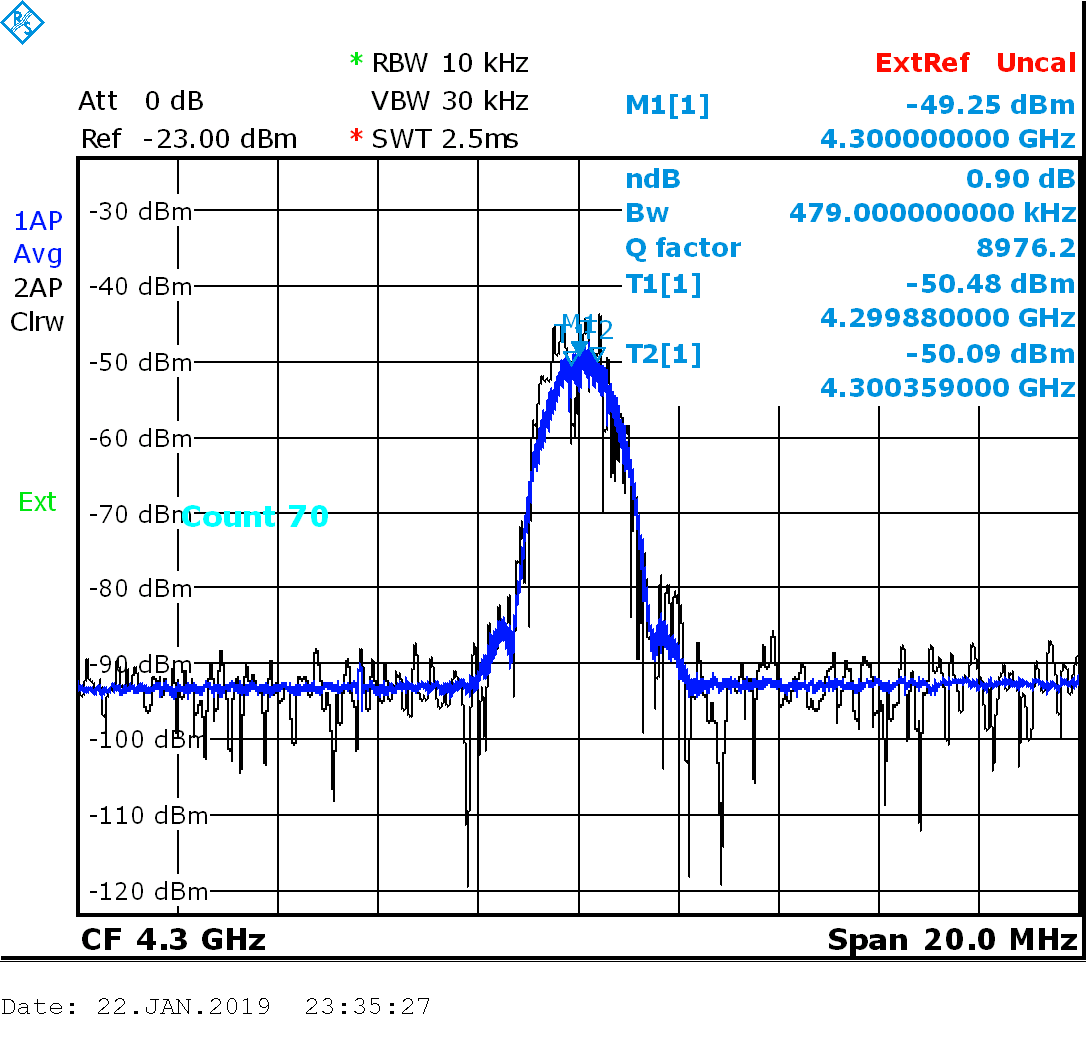
\includegraphics[scale=0.25]{MSK_wvfrm.png}
\caption{MSK Waveform at 4.3 GHz Pictured on a Spectrum Analyzer}

\label{fig:MSK}

\end{figure}

The AFE76 Project Management Committee (PMC) chose the modulation formats to represent candidate WAIC interference. The PMC chose to subject the altimeters to an MSK waveform, as well as OFDM waveforms of varying bandwidths and dual versions of both waveforms. These waveforms were chosen because of their similarity to systems in use for GSM and LTE cellular networks. This meant chipsets were widely available (designed for other frequencies), and WAIC networks could be modeled after purchased IP instead of developed from scratch. Each waveform used ``junk'' data to modulate the carrier, which consisted of randomly generated ones and zeros with equal probability of either.
\subsubsection{MSK Waveform}\label{subsub:MSK}
MSK or Minimum-Shift Keying is a type of modulation format which can be considered as a form of Phase-Shift Keying (PSK) or as a special case of Frequency Shift Keying (FSK)~\cite{proakis_communication_2002}. The frequency separation of an MSK signal, $\Delta f$ is:
$$ \Delta f = \frac{1}{2T}$$
and, thus, it has a modulation index of 1/2. This is ``the minimum frequency separation for orthogonality of the two sinusoids''~\cite{proakis_communication_2002}. An MSK waveform is shown on the spectrum analyzer screen-cap in Figure~\ref{fig:MSK}.

MSK modulation is available natively in the VSG software through the \textit{custom waveform} interface.  The Rhode and Schwarz VSG provides a number of common modulation options in this interface for the user to choose from. This simplifies the waveform generation for this case, as every in-built functionality on the VSG has a SCPI command corresponding to it. 


\subsubsection{OFDM Waveform}\label{subsub:OFDM}

Orthogonal Frequency-Division Multiplexing or OFDM attempts to achieve an efficient, wide-bandwidth communication system by ``dividing the channel bandwidth into equal-bandwidth sub-channels, where the bandwidth of each sub-channel is sufficiently narrow so that the frequency response [...] of sub-channels are nearly ideal''~\cite{proakis_communication_2002}. An OFDM waveform is shown on the spectrum analyzer screen-cap in Figure~\ref{fig:OFDM}.
\begin{figure}[ht]
\centering
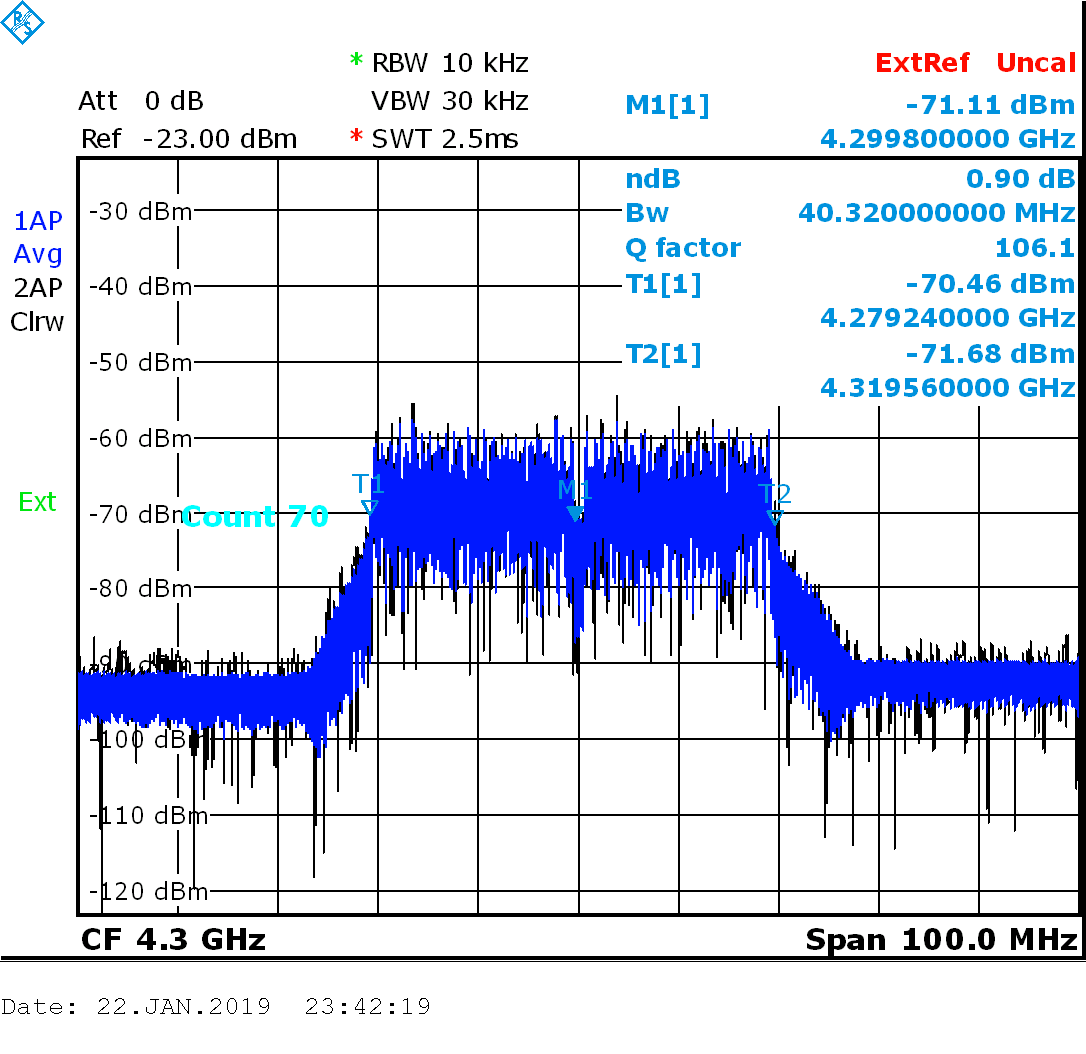
\includegraphics[scale=0.25]{ofdm_wvfrm.png}
\caption{40 MHz OFDM Waveform at 4.3 GHz Pictured on a Spectrum Analyzer}

\label{fig:OFDM}

\end{figure}
One way to view the OFDM waveform is as a series of MSK waveforms spread out orthogonally along a desired bandwidth. From this perspective, MSK can be seen as the minimum bandwidth version of a system based on OFDM, and the altimeter can thus be subjected to wider and wider bandwidth systems to show the response to a greater number of WAIC devices on (or external to) an aircraft. This aspect, as well as the similarity of an OFDM signal to LTE systems, made it a very attractive option for testing the impact of WAIC. 

Generating OFDM signals with the VSG was a more involved process than generating MSK, because the functionality for creating OFDM was not available natively in the VSG software. Consequently, OFDM had to be generated through the VSG's \textit{Arbitrary Waveform Generator}. The arbitrary waveform generator enables the VSG to generate any waveform from IQ data stored in a file on the VSG. The SCPI command for generating an arbitrary waveform must include the file path for this IQ data.  

This enabled an OFDM waveform to be specified by a Matlab script which exports raw IQ data, which is then converted to a form readable by the VSG through proprietary Rhode and Schwarz software. The conversion software allowed the user to adjust the clock rate, thus adjusting the bandwidth of the signal used. The bandwidth could then be measured with a spectrum analyzer to verify the process has yielded the expected waveform. The bandwidth of the OFDM waveform was defined as being 6~dB down from the peak envelope power. 


\subsubsection{Dual Waveforms}\label{subsub:Dual}
The VSG allows full control of an RF generator along with two baseband generators. The RF generator gives the user control of RF carrier frequency as well as the output power level of the carrier in dBm. The baseband generators allow the modulation of two potentially unique waveforms onto the carrier wave, with a possible offset frequency from the center. Both dual MSK waveforms and dual OFDM waveforms of bandwidth less than 40~MHz were tested using a +/-20 MHz offset between them. 

Dual waveforms were considered an important option for testing due to a special characteristic of some altimeters at low altitudes. As the plane descends, the sweep rate of an altimeter increases to give more frequent readings at a more safety critical phase of flight. This is done by significantly reducing the $\Delta f$ covered by the altimeter FMCW. The effects of this offset were thus investigated to determine whether WAIC's impact could be minimized at critical altitudes by leaving the center of the band clear. 


%%%%%%%%%%%%%%%%%%%%%%%%%%%%%%%%%%%%%%%%%%%%%%%%%%%%%%%%%
\section{Python Test Software}\label{sec:Python}
Python code written by the author pieces together the various parts of this setup into an integrated test bench. The goal was to coordinate ARINC 429 signals gathered independently through the Ballard device with signals generated independently using the VSG.
Additionally, software needed to manage large datasets for post processing.
%COMMENT: Above is not a sentence.
Different Python scripts control the various functions of the test bench. These include:
\begin{itemize}
\item Database Creation,
\item Signal Generation,
\item Data Parsing,
\item Time Stamp Coordination,
\item Plotting and analyzing the results.
\end{itemize}

\begin{figure}[ht]
\centering
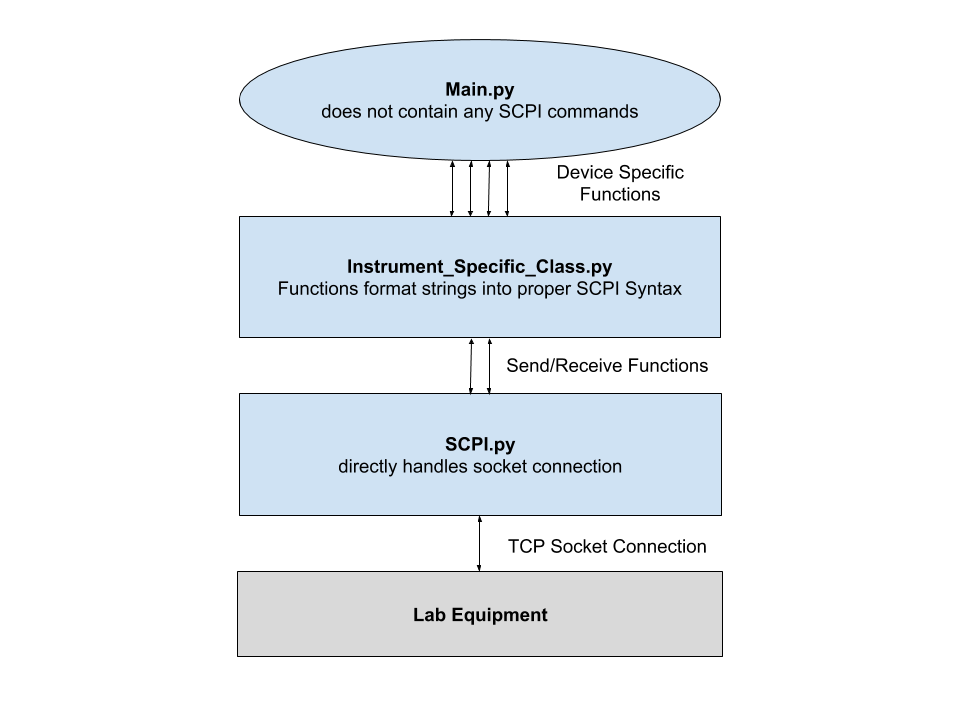
\includegraphics[scale=0.45]{SCPI_Class_Hierarchy.png}
\caption{SCPI Class Hierarchy}
\label{fig:SCPI}
\end{figure}

The software uses Standard Commands for Programmable Instruments or SCPI to control the vector signal generator. In this test bed, the SCPI instructions are processed through an object-oriented hierarchy shown in Figure~\ref{fig:SCPI}. The super-class, SCPI interfaces directly with all lab equipment. The subclass, called \textit{RS\_Signal\_Generator} in this implementation, contains Python functions associated with all instrument specific commands. The helper functions from SCPI send and receive communication with the instrument. Finally, the main loop exists at the highest level, which times the calls of different instrument commands and creates a database to store them. The idea behind this abstraction is to prevent the main loop from dealing with any raw SCPI command syntax -- this should only be handled by one of the instrument classes. 


\subsection{Test Main Loop}\label{sub:mainloop}
The highest level of this design is the test main loop. The test main loop creates the SQLite database which stores all important information for easy transfer between the different Python scripts necessary for the test bed. This program also contains variables for various test parameters, which are stored in an SQLite database for easy reference and sometimes directly control the sequence of a test. Finally, this program loops through the sequence interference signals specified by the various test parameters, and sends the commands to the VSG to generate them. The commands sent to the VSG are time stamped as precisely as possible, and recorded in the \textit{Generated Signals} table in the database. 


Certain test parameters are stored for reference or calculation but do not directly affect the sequence of interference signals to be generated. These include the altimeter make and model, the nominal height of the test setup, the loss experienced by interference signals traveling to the altimeter RX, and the loop loss used in the setup. Other parameters directly control the sequence of the test, including interference on and off times, power levels to be used, modulation formats to be tested, and RF carrier frequencies to be used. 

\subsubsection{Nominal Height vs Correct Height}\label{subsub:nominal}
\textit{Nominal height} is the term used to refer to the approximate altitude determined by the experimental test setup. The difference between measured height and the nominal height of the setup varies between the different altimeters, and is primarily a result of different calibration settings for each altimeter. The calibration procedure is an important part of installing an altimeter onto an aircraft. When an aircraft is on the ground, the TX and RX antennas used by the altimeter are naturally several feet off the ground, in line with the airframe. Additionally, there are standardized delays from the altimeter TX port to the TX antenna and from the RX antenna to the RX port. These are known as Aircraft Internal Delays (AIDs). To compensate for the varying heights of airframes, as well as the AID installation, avionics manufacturers developed a calibration procedure so that each altimeter could be programmed upon installation to output an altitude of 0~ft when the plane is on the ground. 

Because these tests are only concerned with a differential \textit{height error}, rather than the accuracy of an absolute altitude measurement, \textit{nominal height} is only used to set the loop loss. Instead, the baseline measured height with no interference, or \textit{correct height}, is calculated in post processing as the median altitude over a several minute period when the VSG is in the OFF state before the test begins. Any height error attributable to interference is measured as a distortion from this correct height. Because of this, calibration of each altimeter to the setup is unnecessary. 

\subsubsection{Sequence Control}\label{subsub:sequence}
% This section also needs a plot to show the timed stepping up of interference signals. 
The primary purpose of the test main loop is to subject an altimeter to various modulation formats, gradually stepping up the power of each until the altitude readings from an altimeter are distorted or broken. The main loop determines the type of modulation, power level, and timing, and as each signal is turned on or off by the VSG, stores the parameters for the signal in the \textit{Interference Signals} table for use in post processing, an example of which is shown in Table~\ref{tab:Interference}. Each unique modulation format and power combination will have two entries in the \textit{Interference Signals} table, corresponding to the RF ON and RF OFF states of the VSG.  
\begin{table}[]
\centering
\begin{tabular}{@{}cccccccc@{}}
\toprule
ID & Altimeter   & Start Time          & End Time            & Modulation &Carrier Freq& Power & RF State \\ \midrule
1  & Alt A & 19:23:06 & 19:23:07 & MSK & 4300  MHz & -10  dBm & OFF      \\
2  & Alt A & 19:23:07 & 19:23:08 & MSK & 4300   MHz & -10 dBm& ON       \\ \bottomrule
\end{tabular}
\caption{Example Interference Signal}
\label{tab:Interference}
\end{table}

A variety of parameters controls the progression of different interference signals. The \textit{interference\_duration} and \textit{signal\_off\_duration}, define the length of time the altimeter will be subjected to a particular interference signal, as well as the length of time the altimeter will have to recover from any error caused by the previous signal. Throughout the main loop, each signal's Start Time and End time is calculated using interference duration variables. 

A range of RF powers is specified using \textit{power\_min}, \textit{power\_max}, and \textit{power\_step}. For a given modulation format, the main loop iterates through each power level in this range, subjecting the altimeter to this interference power. This allows the user to step through increasing power with as much granularity as is desired for the test.


The final variable, which is important to the progression of a test, is a list called \textit{modulation\_formats}.
This list contains strings corresponding to the different modulations the VSG will generate. MSK and OFDM signals of varying bandwidths will be listed here. The main loop iterates through each string in this list, passing the string to helper functions. 

The first helper function is a lookup which calls the proper function in the VSG class corresponding to a specific modulation format string. The second helper function gives the option for different modulation formats to be put on different carriers, or a list of different carrier functions. Iterating through different carriers for different modulation formats proved to be a critical functionality in later tests.


\subsubsection{Precision of Timing Commands}\label{subsub:timing}
During initial testing phase of the main loop, problems occurred which prevented the \textit{interference\_duration} and \textit{signal\_off\_duration} from precisely controlling the duration and recovery time of an interference signal. This section provides an overview of the different timing issues encountered over the course of these tests, as well as the approaches taken to mitigate each issue. 
 
The first and most serious type of issue encountered while running these tests was termed \textit{hanging delays}. These occurred when the main loop progressed more or less as expected, but the vector signal generator would ``hang'' in its previous state for a significant period of time after the command was sent. 



% Please add the following required packages to your document preamble:
% \usepackage{booktabs}
\begin{table}[]
\centering
\begin{tabular}{@{}ccccccccc@{}}
\toprule
ID & Timestamp   & RF State & Power  & PEP  & Carrier  & Offset 1 & Custom 1 & Arb 1 \\ \midrule
1  & 11:49:39.96 & 1        & -3 dBm & 4.48 & 4300 MHz & 0        & 0        & 1     \\
2  & 12:09:40.26 & 0        & -3 dBm & 4.48 & 4300 MHz & 0        & 0        & 1     \\ \bottomrule


\end{tabular}
\caption{Example VSG State Table}
\label{tab:VSG_State}
\end{table}
 
To address this problem, the program was modified and a new table was added to the database to store the Vector Signal Generator state after each set of commands. Since the purpose of this table was only to be used for debugging, entries were kept as simple as possible. For example, a $1$ in \textit{RF State} corresponds to RF ON, while conversely a $0$ in \textit{RF State} corresponds to the RF OFF setting. The \textit{Power} and \textit{Carrier} columns correspond with the same values in Table~\ref{tab:Interference}. \textit{Offset 1}, \textit{Custom 1}, and \textit{Arb 1} correspond to the state of the first Baseband generator, telling whether the \textit{Custom Waveform Generator} corresponding to a MSK Waveform (see Section~\ref{subsub:MSK}) or the \textit{Arbitrary Waveform Generator} (see Section~\ref{subsub:OFDM}) corresponding to an OFDM waveform are active, respectively. 
 
For the purposes of the timing problem, these attributes serve as a fingerprint, allowing an investigator to correlate each row in the VSG State Table to a row in the Interference Signals table. While information here may seem redundant, this value differs notably from the values in the interference signals table in that the VSG state table is only populated \textit{with values received from the Vector Signal Generator}. Because of this, this table allows for a simple method for looking through the data to find at which point the VSG might ``hang'' in its current state rather than switch to the next signal as specified in the interference signals table. 

Using this method, different theories for potential causes of the hanging delays were investigated. The first potential problem was dropped or delayed packets. During the initial setup, instruments were connected to one another over the TAMU network. While this functioned at a high level, upon packets had an unnecessarily long mean travel time, and significant outliers existed during times of heavy traffic. These issues were solved by moving the VSG and controller laptop onto their own local network. 

 While the local network solved the biggest chunk of hanging delays, it did not eliminate them entirely. These were attributed to a slowdown in the processor handling the sequence of Python commands. These remaining delays would only occur at times of extremely heavy CPU usage (possibly caused by a memory leak in the old Ballard driver), and were eliminated almost completely by rebooting the controller laptop more frequently. Later on, an upgrade to the Ballard driver reduced these even further. 
 
 While the hanging delays were investigated, the VSG State table revealed another source of imprecision in timing commands. It was noticed that the VSG State would not change until nearly a second longer than the \textit{Interference Duration} or \textit{Signal off Duration} parameters specified. This drift occurred because the main loop used Python in-built \texttt{Sleep()} function to handle timing. The sleep function used the exact interference duration passed as a parameter. After the program `woke up', the commands to set the next interference signal up would be called, thus introducing a small delay beyond the specified duration. 
 
 This problem was dealt with by replacing the \texttt{Sleep()} function with a custom function called \texttt{Wait\_Until()}. This new function takes the signal end time as a parameter (see Table~\ref{tab:Interference}), subtracts the current time from the end time, and uses the new value as the parameter for Python's in-built sleep function. This allows the next end time to be calculated in advance by adding the \textit{Interference Duration} or \textit{Signal off Duration} to the previous signal's end time, and storing the previous signal's end time as the start time for the next signal. %[This section definitely could use some sort of diagram...]

Using the \textit{wait until} method to time commands offered important new flexibility to the main loop. This method allows writing signals to a database, setting up the baseband generators, and pinging the VSG for the VSG State information all to occur while the VSG is in an RF OFF state. While the VSG settings cannot be adjusted in RF ON while maintaining the integrity of the signal, writing to the database and pinging the VSG for state information can also be done during this state, and the \textit{wait until} function will still wake the program at the proper time to turn the VSG on or off. The implementation of the \textit{wait until} function eliminated the drift problem, and allowed for the \textit{Interference Duration} and \textit{Signal Off Duration} parameters to precisely control the signal on and off time. 

\begin{figure}[ht]
\centering
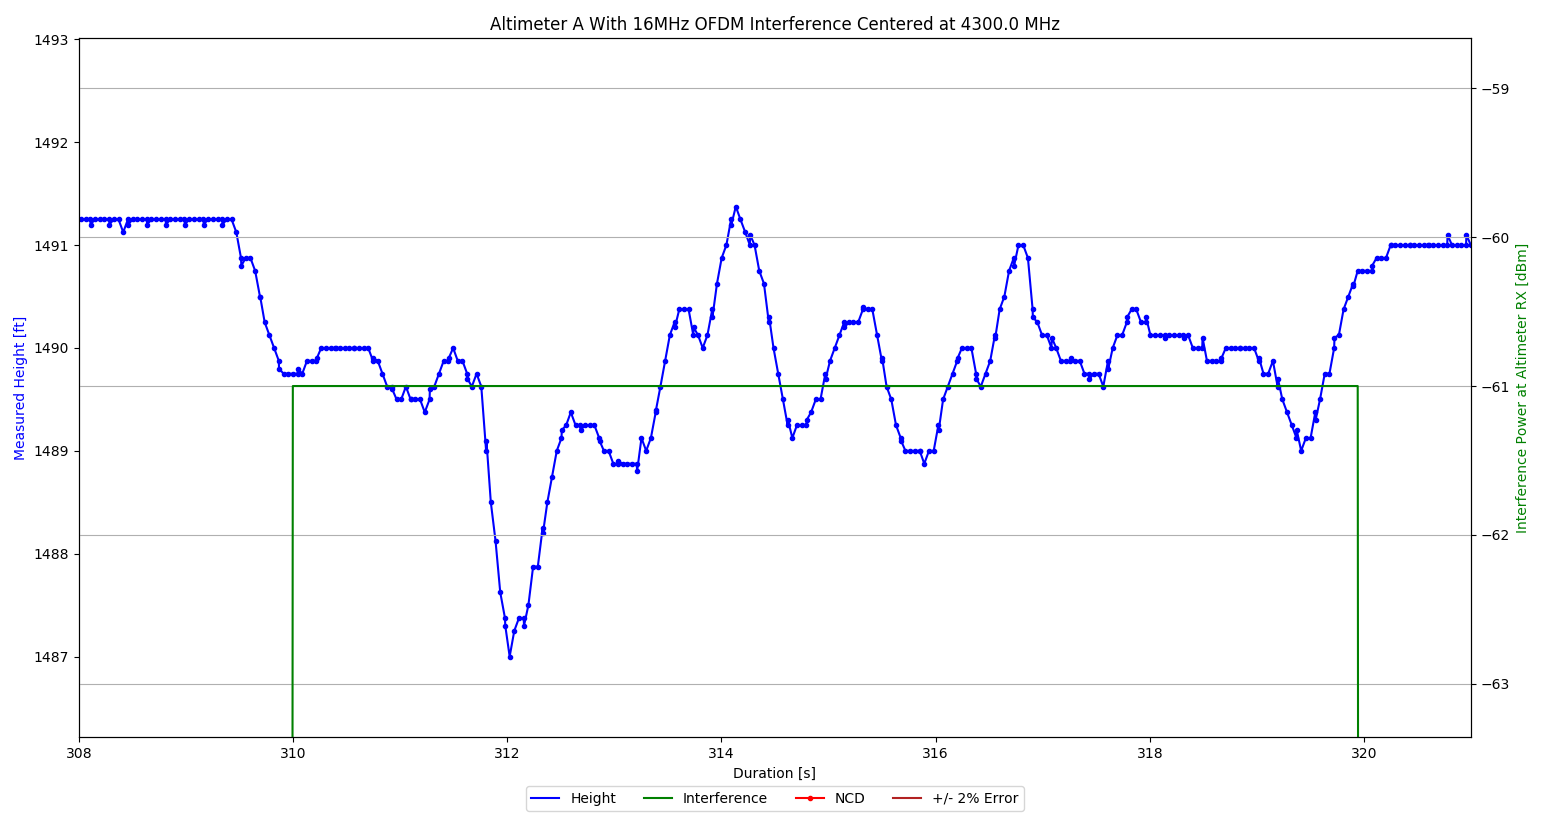
\includegraphics[width = 6 in ]{sync_err.PNG}
\caption{Height Plot Showing Sync Error}

\label{fig:sync}

\end{figure}
The final problem encountered involved the synchronization of time stamps of data between the controller laptop and the Ballard ARINC device. The Ballard internal clock drifted from about half a second ahead of the controller laptop clock to about half a second behind. This led to data sets such which looked like Figure~\ref{fig:sync}, where distortion from the correct height would appear a split second before the interference signal was turned on. Additionally, due to averaging techniques used in the altimeter's signal processing, there would be several data points during which the altitude would recover from the distortion caused by any interference. 


While this issue could not be fixed completely, several different approaches were taken to mitigate it. Firstly, the Ballard used in initial testing was an older unit, which meant it was more prone to clock errors. To address this, the clock was driven by an external IRIG-B timecode signal, rather than the on board IRIG~\cite{noauthor_overview_2017}. A program called NMEA time generated the IRIG signal through the controller laptop's audio jack, which was then fed into the Ballard input.  These changes would not completely synchronize the Ballard, but it would limit the drift of one clock away from another throughout a test. 


Later on, when a new Ballard was purchased for this project, the external IRIG signal was no longer needed, as the updated Ballard driver provided adequate synchronization over USB. Another technique used to prevent any loss of synchronization was to periodically power cycle the Ballard to ensure that the clock is reset. Finally, to minimize the impact of any data points not captured in the RF ON interval by post processing, long interference durations were used to ensure that the impact of any missed points on the true average was minimized. 

\subsection{VSG Class}
The VSG Class allows the main loop to create an object corresponding to each VSG connected to the network in the lab setup. This object then has access to functions which perform every operation needed by the main loop. The VSG Class inherits functionality from \textit{SCPI.py} common to every SCPI programmable instrument. The VSG class provides functionality for controlling both the RF generator, as well as the VSG's two baseband generators. 

The general purpose of each function in the VSG class is to construct the string for each SCPI command corresponding to that function, and send the command using the inherited SCPI \textit{send} function. For example, the following SCPI command sets Baseband A to MSK modulation:
\begin{center}
\textit{``SOUR1:BB:DM:FORM	MSK.''}
\end{center}
``SOUR1'' corresponds to baseband generator A, where ``SOUR2'' would correspond to baseband generator B. Different SCPI commands have different parameters like this which the VSG class takes in as a normal Python variable and inserts into the string. 

The VSG class provides several functions which perform this task for the RF Generator. RF ON and RF OFF commands are self explanatory, while the \textit{set\_carrier} function lets the user choose a carrier frequency as well as the RF power setting.

Similarly, the VSG class offers functions which will set the custom modulation format of either baseband generator (for setting MSK), or for setting the arbitrary waveform generator in each baseband generator (for setting OFDM). This class also provides functions for enabling and disabling the baseband generators, which is necessary for switching between dual and single modulation formats. 

Lastly, the VSG class will have functions for setting a dual MSK or dual OFDM waveform. These will make two calls to the single MSK or OFDM function within VSG, simply passing a different source parameter to specify a different baseband generator.  

\subsection{SCPI Class}
\textit{SCPI.py} contains the `lowest' level of programming in the SCPI hierarchy shown in Figure~\ref{fig:SCPI}. The goal of this abstraction was to implement a small set of core functionality that would be needed for any instrument capable of running SCPI commands. The SCPI class handles the TCP connection, sends and receives all commands and queried data from the instrument, and contains a few other universal instrument commands. 

The first task handled by SCPI is the initialization of the socket connection between the controller laptop and the instrument. The constructor takes in the IP address of the instrument and the port number, and uses the Python socket class to initialize the connection. When the experiment is over, the SCPI \texttt{close} function which handles the proper termination of the socket connection. 

Next, the SCPI class creates custom send and receive commands inherited by every instrument object. The send command handles the proper encoding of any SCPI command string before calling the native socket class \texttt{send} function. The receive command decodes a received string from the instrument, and parses the string into the different array elements delimited by commas in SCPI syntax. The receive command is meant to be called within any subclass command which \texttt{queries} the instrument for information, as the data types received will vary depending on the query. 

Finally, there are a few other commands universal to almost every SCPI controlled device. The \texttt{reset} command ensures the instrument begins each experiment from a clean state. The \texttt{operation complete} query is called between commands to ensure that no commands are executed out of order. Last, the \texttt{identify} query returns the instrument make and model information, which is useful when first setting up an instrument for automation. 

\subsection{Post-Processing}
After the test sequence is completed, a series of other Python scripts are used to post process the newly generated data. Time stamped altitudes must be exported from the Ballard CoPilot software into an Excel document, and a python script has to read the data from this log into the SQLite database. A second program uses the time stamps from both the logged altitude table and the generated signals table to create a full data set, where each altitude measurement is labeled with the type and magnitude of interference the altimeter was subjected to at that time. Finally, several Python scripts take this full dataset and use it to generate plots which aid in the interpreting of the results. 

\subsubsection{Parsing The Copilot Log}
The first post processing script parses the Ballard Copilot log into the SQLite database so that it can be used by other scripts. The CoPilot export is in an excel file formatted like Table~\ref{tab:Copilot}. This table is read by python using SQLite's built in \texttt{read\_excel} function. Most of the data is then added to the SQLite database as is, but the \texttt{Value} string is stripped of units and cast as a float so that the numerical value can be easily used by other scripts. 

The most important columns are the \texttt{Value}, \texttt{Time}, and \texttt{Activity} label. The Activity label reads `SSM ERROR'  whenever the altimeter does not receive a strong enough signal to make a reliable altitude calculation. Points with this flag are called NCD or Non-Computed Data. 
\begin{table}[]
\centering
\begin{tabular}{ccccccc}

\hline
Item \# & Ch\# & Lbl\# & Value    & Time    & Activity      & Name         \\ \hline
0       & 0    & 165   & 509 feet & 26:45.4 & LO            & Radio Height \\
1       & 0    & 165   & 509 feet & 26:45.5 & LO SSM ERROR & Radio Height \\ \hline
\end{tabular}
\caption{Example Copilot Export}
\label{tab:Copilot}
\end{table}

\subsubsection{Mapping Interference Signals to Copilot Data}
The next post processing script maps each of the Altitude data points from the copilot log (Table~\ref{tab:Copilot}), and maps them to the interference signal (Table~\ref{tab:Interference}) active at that time. The method for mapping them is simple: if the time stamp for the data point is greater than an interference signal's \textit{start time} and less than the same interference signal's \textit{end point}, the altitude data is labeled with the corresponding modulation format, RF Power, RF State, and Altimeter under test information from the interference signals table. This process is repeated until all data points have been mapped. 

% Please add the following required packages to your document preamble:
% \usepackage{booktabs}
\begin{table}[]
\centering
\begin{tabular}{@{}ccccccclll@{}}

\toprule
ID & Timestamp  & Ch\# & Carrier& Altimeter & Height & Modulation  & Power& Status & RF \\ \midrule
0  & 13:54:40.5 & 0    & 4300              & Alt A     & 506             & 80 MHz OFDM & 7               & LO     & ON       \\
1  & 13:54:40.6 & 0    & 4300              & Alt A     & 506             & 80 MHz OFDM & 9               & LO     & OFF      \\ \bottomrule
\end{tabular}
\caption{Example Full Dataset Table}
\label{tab:Full}
\end{table}

%%%%%%%%%%%%%%%%%%%%%%%%%%%%%%%%%%%%%%%%%%%%%%%%%%%%%%%%%
\section{Initial `Waic Only' Test Plan}\label{sec:initial}
The test setup design described above gave a wide degree of flexibility to the type, magnitude, and timing of interference the altimeters could be subjected to. While some preliminary tests helped to develop and debug the test setup, these were not comprehensive enough to draw conclusions from. This covers the development questions of for and the execution of the first  comprehensive test regimen. Additionally, this section pieces together the components discussed earlier into a complete test diagram. 

\subsection{Motivations}
The initial testing regimen had a series of questions about the behavior of real altimeters in the presence of interference that needed to be answered: 

\begin{itemize}
\item At what power level will \textit{any} MSK or OFDM signal at 4.3 GHz `break' an altimeter?
\item Does the `breaking point' an altimeter depend on the bandwidth of the signal?
\item Does adding separation between interference signals at the center influence the `breaking point'? 
\item How does the positioning of a signal within the altimeter band affect the breaking point?
\item The \textit{definition} of precisely what `breaking point' means in the context of these tests also needed development.  
\end{itemize}

A discussion of preliminary testing between the PMC and the author in the context of these driving motivations led to development of the methods discussed in earlier sections which culminated in the test procedure discussed here.  

\subsection{Complete Diagram}
While the diagram of the Modified Test Setup in Figure~\ref{fig:Modified} gives conceptual background to the tests, and Figure~\ref{fig:Altitude_Simulator} gives detailed insight into the operation and configuration of the altitude simulator, neither is detailed enough to provide the context necessary for a complete test description. Figure~\ref{fig:Initial} shows the full test setup used in detail. A full page version is provided in Appendix~1. 
% COMMENT use ref structure for Appendix



\begin{figure}[ht]
\centering
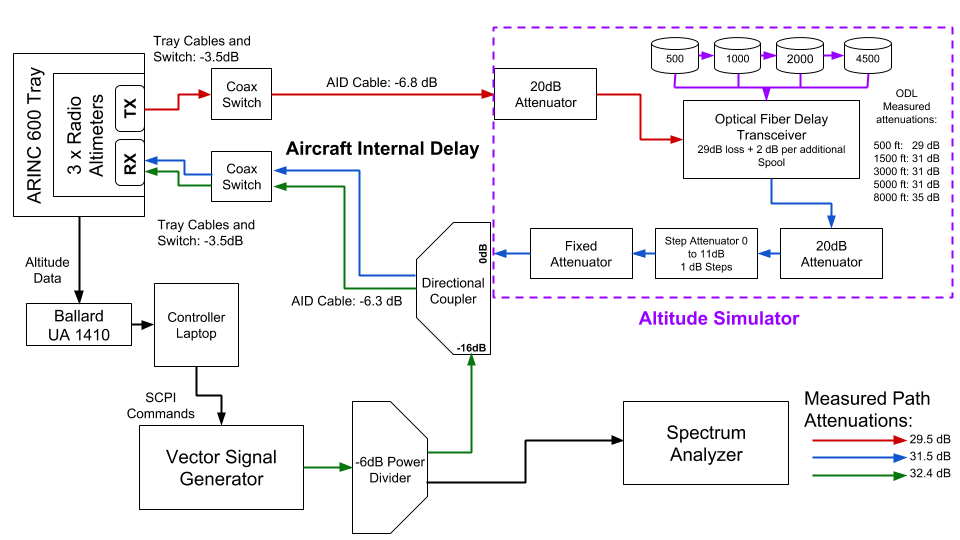
\includegraphics[width = 6 in ]{Initial_Full_Setup.PNG}
\caption{Full Test Bench Diagram for Initial Tests}

\label{fig:Initial}
\end{figure}

This diagram shows the altitude simulator  embedded into the full test setup, as well as measured path attenuations with the step and fixed attenuation set to zero. The measured path attenuations are then used to determine a value for the fixed attenuator (10,20, or 30dB), and a value for the step attenuator (1-11dB) to precisely achieve the DO-155 specified loop loss between TX and RX. Table~\ref{tab:loop loss} shows the loop loss values used for the different heights in this setup. 

For 500~ft, which had the lowest attenuation, the loop loss from TX to RX was just within the dynamic range of a network analyzer, and so could be verified experimentally with a single S21 measurement. Higher altitudes could not be verified in this manner, but because the measurement closely matched calculations for 500~ft, extrapolating to higher altitudes and loop losses was reasonable. 

Several elements not shown in the conceptual diagram from Figure~\ref{fig:Modified} are added in Figure~\ref{fig:Initial}. The output of the VSG is divided between the interference injection point and a spectrum analyzer using a 6~dB resistive coupler. The spectrum analyzer allows the test operator to view the interference signals actively being tested, and make adjustments to the setup when they do not match expectations. A directional coupler allows interference to be inserted into the altimeter line at the injection point without adding additional attenuation to the loop. 

 Other elements pictured which weren't on the original diagram include coax switches and an ARINC 600 tray. The tray and switches are necessary in part because the DC power supply to each altimeter is different, and the tray acts as a protection from damage. Additionally, they allow for quick and easy alternating between the various altimeters under test, which is important in case any of this is ever actually flight tested. 

\subsection{Breaking Point Definition}

The purpose of these tests was to search for an altimeter's `breaking point' under various scenarios of interference. Performance standards for radio altimeters first set out in DO-155 were updated in the ARINC 707 standards~\cite{noauthor_arinc_2009}. The standards stated that ``radio altimeter accuracy, when measured in accordance with RTCA DO-155, [should] be within 1.5 feet or 2\%, whichever is greater.''  WAIC or out of band interference needed to demonstrate that it distorted the altitude signal less than these standards. Thus, the breaking point was defined as either a) a maximum height error beyond the 2\% or 1.5 feet allowable by ARINC 707, or b) any height reading labeled NCD. 

\subsection{Test Definition}
\begin{table}[]
\begin{tabular}{c|c|c|c|c|c|c|c|c}
\multicolumn{4}{c|}{\textbf{Interference Signal}}   & \multicolumn{3}{c|}{\textbf{VSG RF Power}} & \multicolumn{2}{c}{\textbf{Power Durations}} \\
Modulation & Bandwidth & Center   & Offset & Min         & Step    & Max       & ON                & OFF              \\ \hline
MSK        & 5 MHz     & 4300 MHz & 0 MHz  & -60 dBm     & 2 dB    & 10 dBm    & 10 s              & 10 s             \\
Dual MSK   & 5 MHz     & 4300 MHz & 20 MHz & -60 dBm     & 2 dB    & 10 dBm    & 10 s              & 10 s             \\ \hline
OFDM       & 5 MHz     & 4300 MHz & 0 MHz  & -60 dBm     & 2 dB    & 10 dBm    & 10 s              & 10 s             \\
Dual OFDM  & 5 MHz     & 4300 MHz & 20 MHz & -60 dBm     & 2 dB    & 10 dBm    & 10 s              & 10 s             \\ \hline
OFDM       & 10 MHz    & 4300 MHz & 0 MHz  & -60 dBm     & 2 dB    & 10 dBm    & 10 s              & 10 s             \\
Dual OFDM  & 10 MHz    & 4300 MHz & 20 MHz & -60 dBm     & 2 dB    & 10 dBm    & 10 s              & 10 s             \\ \hline
OFDM       & 20 MHz    & 4300 MHz & 0 MHz  & -60 dBm     & 2 dB    & 10 dBm    & 10 s              & 10 s             \\
Dual OFDM  & 20 MHz    & 4300 MHz & 20 MHz & -60 dBm     & 2 dB    & 10 dBm    & 10 s              & 10 s             \\ \hline
OFDM       & 40 MHz    & 4300 MHz & 0 MHz  & -60 dBm     & 2 dB    & 10 dBm    & 10 s              & 10 s             \\
OFDM       & 80 MHz    & 4300 MHz & 0 MHz  & -60 dBm     & 2 dB    & 10 dBm    & 10 s              & 10 s            
\end{tabular}
\caption{Test Definition For Initial Testing Regimen}
\label{tab:initial_signals}


\end{table}
Table~\ref{tab:initial_signals} shows the interference signals used for one of the last runs of the initial testing regimen. This test definition was the result of a year and a half long process of expirimentation with the test setup.Tests expirimented with loop loss settings, investigated the ARINC429 synchronization issues, investigated the relative sensitivity of different portions of the band, and investigated the bandwidth dependence of interference signals. The results of the earlier tests are summarized here, while the test definition from Table~\ref{tab:initial_signals} is used as a representative example. 

Early tests experimented with the position from which loop loss was to be measured. There was an argument that the loop loss should be measured between the terminals of the altitude simulator rather than the terminals of each altimeter. This was abandoned when multiple altimeters were unable to acquire an altitude signal with the higher loop loss. This led to the values from Table~\ref{tab:loop loss} of attenuation between altimeter terminals being finalized. Investigations into the measurement syncronization issue were covered in depth in Section~\ref{subsub:timing}.

 Another early test procedure investigated which portion of the radio altimeter band was most sensitive to interference. OFDM signals of the same bandwidth were placed at varying center frequencies to test the altimeters' sensitivity to band placement. These tests confirmed the hypothesis that the center of the radio altimeter band was the most sensitive to interfering signals. 

Finally, the test regimen shown in Table~\ref{tab:initial_signals} was used to systematically investigate the sensitivity of the radio altimeters to different bandwidths of interference. These signals were used across all altimeters under test, and across all altitudes the optical delay line could produce in Table~\ref{tab:loop loss}. The results are discussed in Section~\ref{sec:initial_results}.

%%%%%%%%%%%%%%%%%%%%%%%%%%%%%%%%%%%%%%%%%%%%%%%%%%%%%%%%%
\section{Expanding the Test Setup}\label{sec:expanding}
The results from the initial test regimen led to new avenues of investigation. The dependence of results upon the bandwidth occupied by interference signals led to a need for wider bandwidth signals in the test bed. A desire to present the worst possible case for an aircraft led to testing at lower altitudes with interference from other altimeters. This simulated an approach or takeoff scenario at a busy airport. Finally, developments in 5G communications lobbying for access to adjacent bands led to an investigation of the tolerance of real altimeters to out of band interference. All of this required modifications to the initial testing concept from Figure~\ref{fig:Modified} to couple in an extra VSG and simulated altimeter signals at the interference injection point (Figure~\ref{fig:Wideband}).
\begin{figure}[ht]
\centering

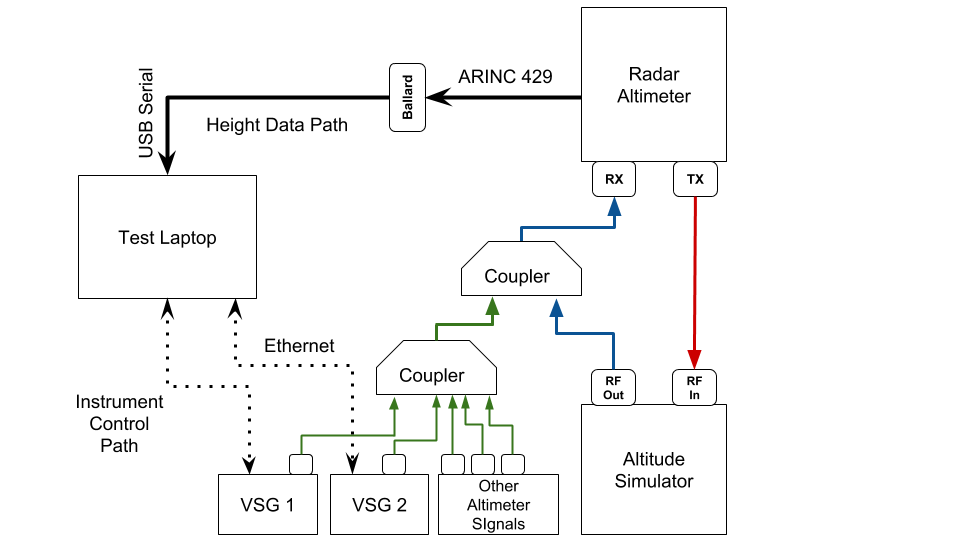
\includegraphics[scale=.5]{Wideband_Test_Setup.png}
\caption{Expanded Test Bench For Wideband and Altimeter Interference.}

\label{fig:Wideband}

\end{figure}
\subsection{Adding The Second VSG}
Early testing clearly demonstrated the effects of interference bandwidth on the altimeter signal processing. Wider bandwidth OFDM signals caused the altimeter to break at a lower RF Carrier power than narrower bandwidth signals. This dependence made it necessary to demonstrate the effects of OFDM filling the entire 4200 to 4400~MHz band (see Section~\ref{} Results of initial testing).
% COMMENT FIX THIS!
However, the Rhode and Schwarz SMU 200A VSG used for initial testing could only support an 100~MHz OFDM signal due to bandwidth limitations on the instrument.  

To supplement this, a Rhode and Schwarz SMW 200A was located in the senior design lab, and was appropriated (with permission of the owner) for the purpose of expanding the testing capability. This slightly newer VSG could support a 160 MHz OFDM signal, and when used in conjunction with the first VSG, the two filled the full spectrum. A secondary goal of this process is to test the effects of proposed cellular networks in adjacent bands to the altimeter band while still maintaining simulated WAIC Interference. The dual VSG setup allowed for the one VSG to simulate in band interference while the other swept through out of band signals. 

\subsubsection{Providing Isolation to the VSGs}
\begin{figure}[ht]
\centering
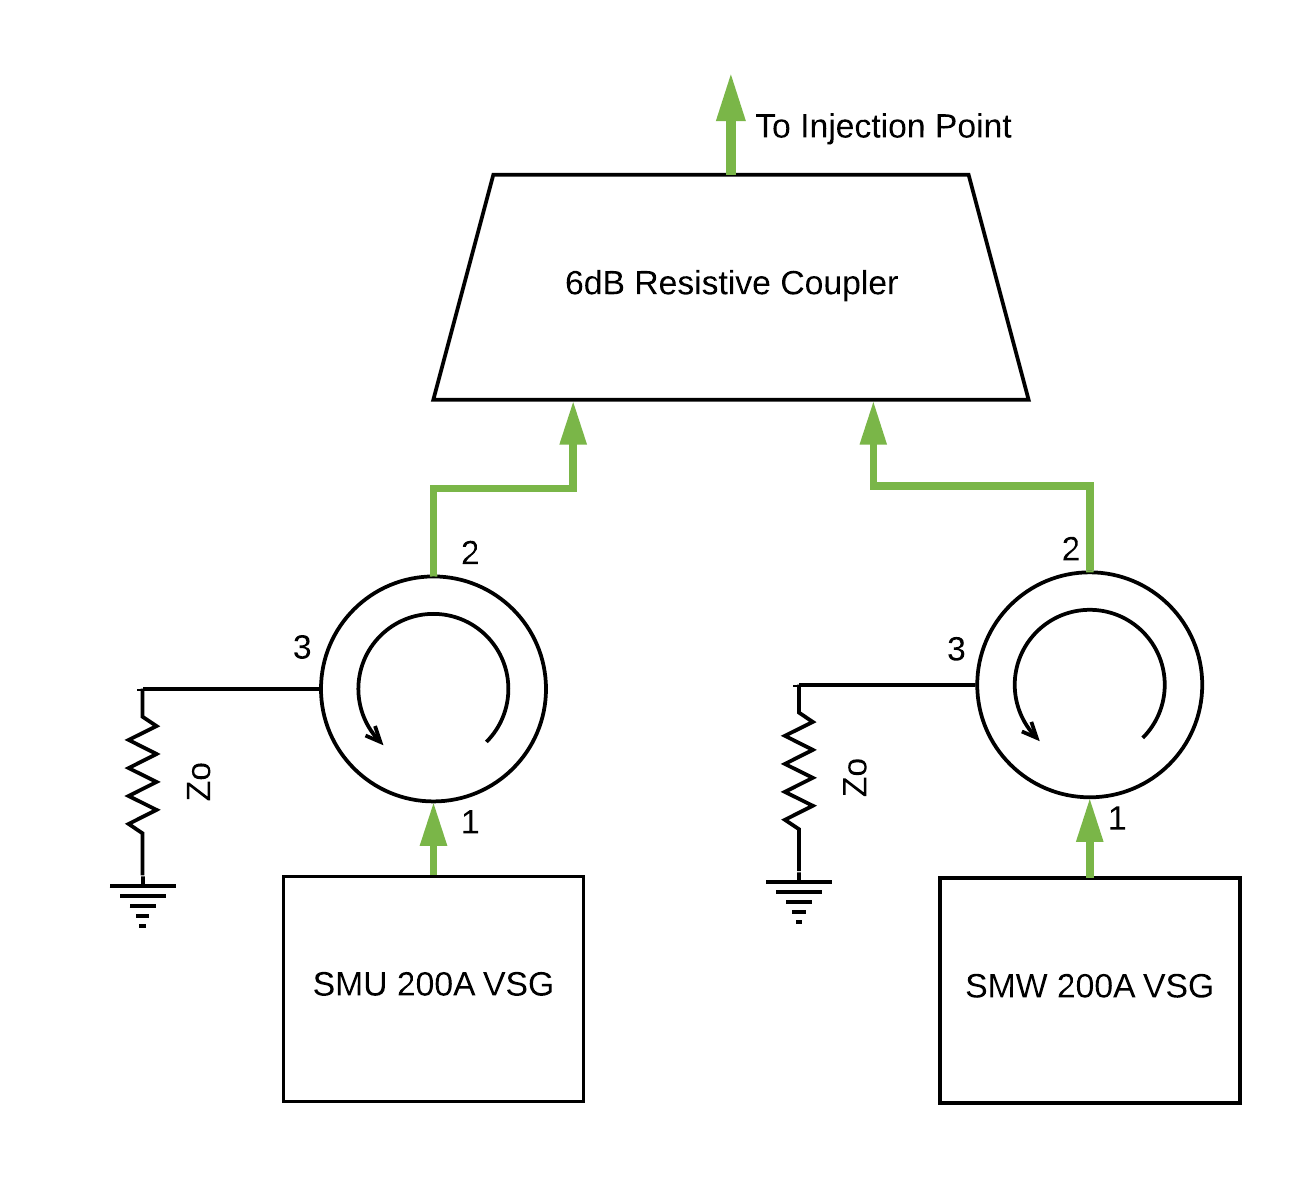
\includegraphics[scale=1]{Isolators_Coupler.PNG}
\caption{Circulator with Matched Load Added to Protect VSGs}

\label{fig:circulator}
\end{figure}
One problem with using the 6~dB resistive power divider to couple the interference from the two VSGs together was the lack of isolation. The coupler provides no directionality, and signals which enter one port are split equally between the two other ports. This was hazardous since the high interference powers being tested could damage the other VSG if fed into the \textit{RF Out} port in reverse. 

AVSI began looking into purchasing other couplers to provide higher isolation to the VSGs, when the Garmin engineer participating in the project offered to contribute two circulators which could function as isolators. By placing a matched load at port~3, most power entering from port~2 is absorbed into the load, with very little (ideally none) reflected back to port~2 or allowed to pass to port~1. Signals entering port 1 experience a small attenuation due to the properties of the circulator. Figure~\ref{fig:circulator} shows how circulators in this configuration provide isolation to the VSGs when coupled together. 

\subsubsection{Achieving Higher Power Interference}

\begin{figure}[ht]
\centering
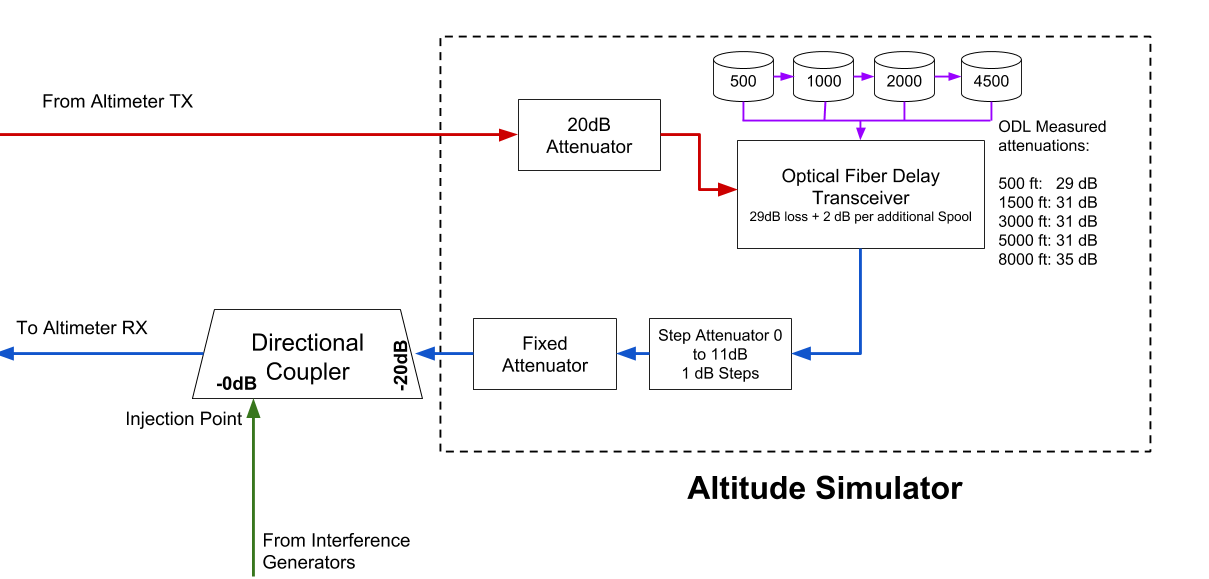
\includegraphics[width = 6 in]{Coupler_Swap.png}
\caption{Modifications for Higher Interference Power}

\label{fig:coupler_swap}

\end{figure}


While the isolators protected the VSGs from damaging one another, they also added more attenuation into the line, meaning the altimeter RX received a lower RF Power than in earlier tests. This upper limit, caused by the Peak Envelope Power (PEP) limitation of the VSGs, prevented tests from locating the breaking point of an altimeter sometimes. 


The setup was modified again to fix this. The 20~dB attenuator placed on the output of the optical delay line in the altitude simulator was removed, and the 16~dB directional coupler was replaced with a 20~dB directional coupler. Figure~\ref{fig:coupler_swap} shows how the output of the altitude simulator fed into the 20dB loss port of the directional coupler to compensate for removing the fixed attenuator, and the interference injection point was moved to a port with (ideally) no attenuation. Additionally, this configuration was advantageous because the step attenuator and variable fixed attenuator settings for different altitudes did not have to be recalculated. 

A Vector Network Analyzer S21 measurement was taken to verify the isolation provided by this configuration, as well as the attenuation between each VSG RF port and the altimeter RX. 

\subsection{Simulating Altimeter Interference}
The other major modification shown in Figure~\ref{fig:Wideband} was the addition of other altimeter signals to the interference already being tested. This addition intended to move the setup closer to the real-life worst case scenario for the interference an altimeter might be subjected to. The test bed was configured to replicate an approach for landing scenario used in earlier compatability investigations. A series of VCOs were calibrated and driven by function generators to generate the external altimeter signals, and programmable and fixed attenuators configured the distance of each altimeter signal from the receiver. The VSG setup was configured to simulate the interference of the full 4.2 to 4.4 GHz band filled with WAIC signals from other aircraft, with a goal of determining what WAIC radiated power limitations were necessary to protect altimeters. Finally, all of these signals were coupled together with the VSG signals to send toward the interference injection point. 


\subsubsection{Determining the Worst-Case Scenario Geometry}
A worst-case scenario for the interference experienced by a victim altimeter from other aircraft was developed in the 2014 compatibility studies submitted to the ITU~\cite{noauthor_compatibility_2014}. The authors determined that the altimeter data was most important to the safety of a flight during the landing phase of operation. When aircraft line up for approach, they typically maintain a distance of around 5~km, which makes interfernce from WAIC signals or other altimeters aboard these neighbors negligible. On the other hand, aircraft taxiing or in holding adjacent to a runway can achieve distances less than 300~m to the victim RA. These aircraft could present a significant hazard to nearby altimeter receivers if WAIC power limitations are not developed in the context of this scenario. 

\begin{figure}[ht]
\centering
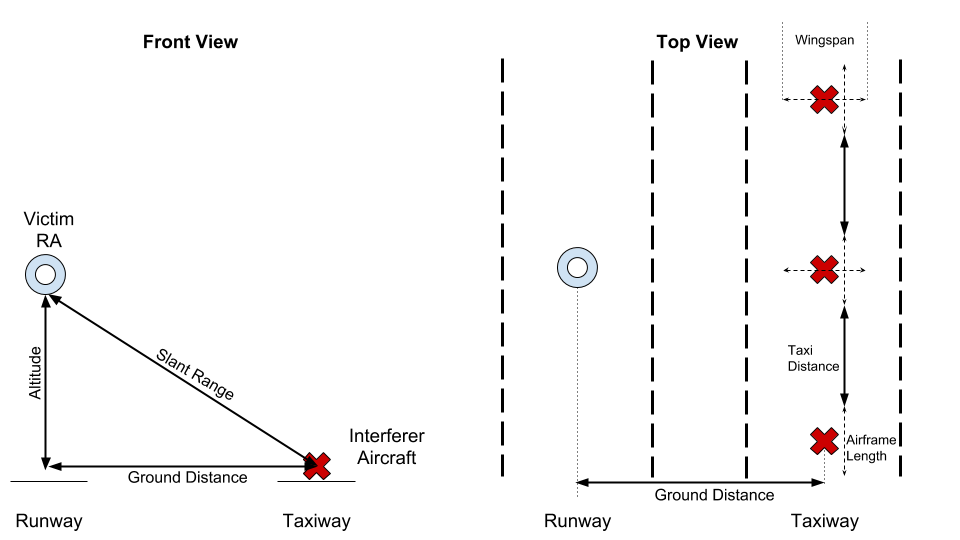
\includegraphics[width = 6 in]{Victim_RA.png}
\caption{Geometry Used in ~\cite{noauthor_compatibility_2014} for Interference During Landing Scenario}

\label{fig:victim_ra}

\end{figure}

Figure~\ref{fig:victim_ra} shows the geometry from~\cite{noauthor_compatibility_2014} which was also used for the this compatibility study. The markers represent the center of the airframe for each aircraft. Three parameters specify the distance of aircraft to one another in this scenario. The \textit{ground distance} between the runway and adjacent taxiway, the \textit{altitude} of the victim aircraft during descent, and the \textit{taxi distance} from nose to tail of aircraft in the queue for takeoff. A \textit{slant range} between the victim RA and an interferer can be determined using these parameters. Additionally, the \textit{wingspan} and \textit{airframe length} of each plane plays a role in the location of potential interferers.

The path losses from simulated WAIC signals were calculated in the context of this geometry. Altimeter transmitters and receivers were located at the center of the airframe, directly underneath each aircraft. Interferers modeling WAIC devices for applications internal to the aircraft were grouped together at the center-point inside of each airframe. For applications external to the aircraft, Interferers were grouped together at the wing tip closest to the victim altimeter. This model provides a worst case scenario for WAIC interference, because in reality WAIC devices would be distributed throughout an airframe according to the need of an application, rather than grouped together at the point closest to an external aircraft's receiver. 
%	
%	Initially, the authors attempted to model all WAIC devices as omnidirectional point sources (OPS's)~\cite{noauthor_compatibility_2014}. This model is simple yet provides a relatively accurate accounting for the pattern given off by antennas at large distances. However, the OPS model assumed homogeneous radiation in every direction. The authors found that external WAIC devices violated the protection criteria for incumbant services in the band. To mitigate this, a radiation pattern was applied which limited power in critical directions. 

%	While the aforementioned study focused primarily on WAIC interference, 
In addition to specifying the path loss experienced by WAIC interferers located at a minimum slant range, this geometry also served to model the interference subjected to the victim RA by other altimeters. While most altimeters are designed to handle external altimeter signals, the \textit{combination} of these signals with WAIC interference leads to more stress on the victim receiver. This geometry models the locations of external altimeters along with WAIC signals to simulate this effect. Path losses assigned to each simulated altimeter are specified by the location in this geometry. 

\begin{figure}[ht]
\centering
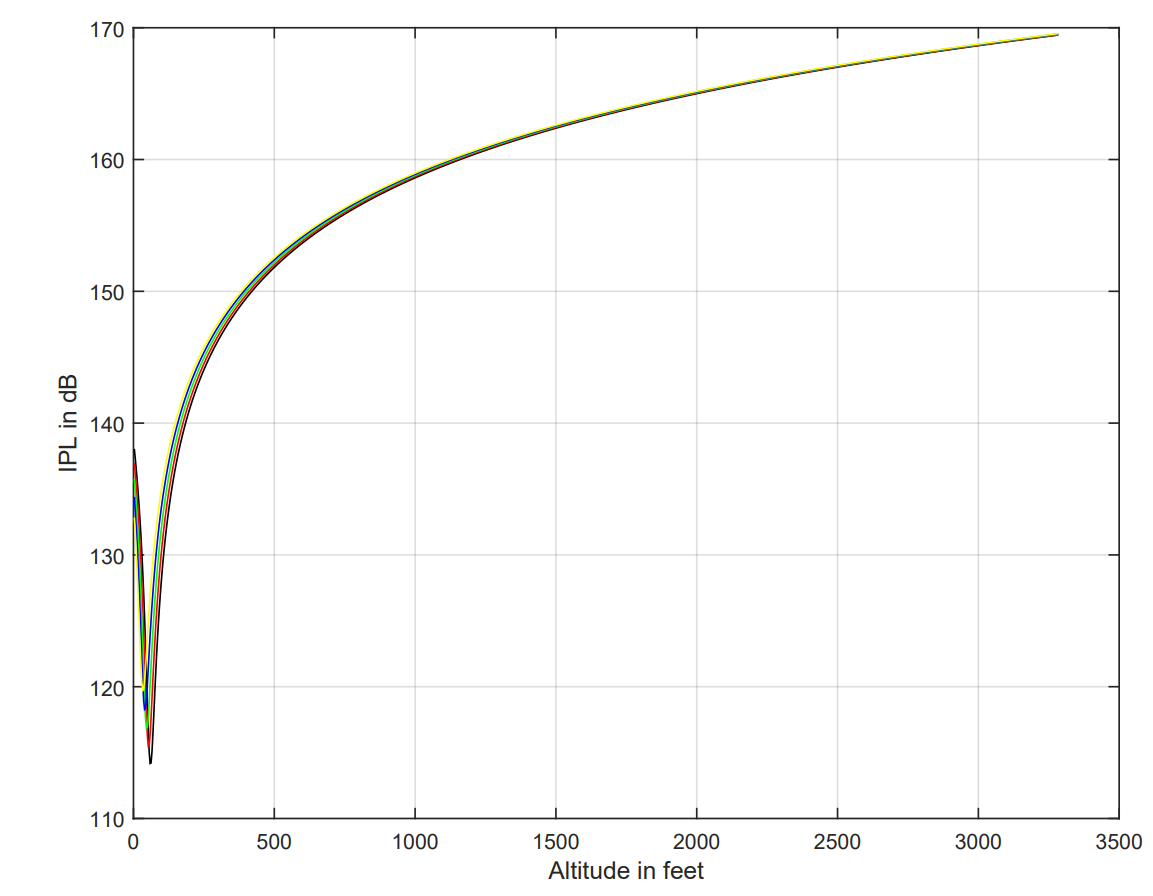
\includegraphics[scale=.6]{IPL_Plot.png}
\caption{Plot of IPL values for 15 closest aircraft}

\label{fig:IPL}

\end{figure}

The geometry was then modeled in a Matlab script by Airbus as a contribution to this project. The victim aircraft approached for  a landing on a 3 degree glide slope, and the interference path loss (IPL) from each aircraft on adjacent taxiways were modeled  in the script. Figure~\ref{fig:IPL} shows the results of this analysis. The IPL value for each of the 15 nearest aircraft are shown as a function of height, with a minimum occurring at approximately 200~ft due to the angle of of reflected interference signals offering the shortest direct path into the victim RX antenna. From this, the committee drew the conclusion that the worst case altitude for this geometry occurred at approximately 200~ft. 

However, the lab test equipment had available test altitudes of only 40 and 500~ft. After some deliberation, the 500~ft altitude was chosen for the approach tests. By configuring the IPLs for the 200~ft case, and the altimeter loop loss for a 500~ft case, the signal to interference ratio went from the real life worst case scenario to a so-called `super' worst case scenario: $$\frac{S(200ft)}{I(200ft)}\leq\frac{S(500ft)}{I(200ft)}.$$
This super worst case would be used to configure interfering altimeters for the landing simulation.


\subsubsection{Simulating Individual Altimeter Signals}
Several approaches were considered to simulate altimeter signals for the approach scenario. While software defined radios were appealing for the convenience the offered in modifying the test bed, they were in the end rejected in favor of a series of Voltage Controlled Oscillators (VCOs) controlled by function generators. The major advantage seen in the VCO approach was the simplicity of explaining the test scenario to regulators, as opposed to having to present another piece of software.

Eight two-channel function generators and 16 VCOs were ordered for this purpose. The function generators were configured to output a triangle voltage wave to drive the VCOs in the FMCW pattern seen in Figure~\ref{fig:FMCW}. The min and max voltage on the triangle wave correspond to the VCO setting for the min and max frequency of the simulated altimeter waveform. The frequency of the voltage waveforms was varied between different VCOs to simulate the varying pulse frequencies exhibited by different altimeters as well as to provide randomness to the simulation. It was considered critical that the different simulated altimeter signals were asynchronous to provide a realistic scenario. 


\subsubsection{Connecting the VCO Signals}
Figure~\ref{fig:VCO_Coupler} shows how the VCO signals were coupled together to simulate 16 different altimeter signals. While the initial plan had been to simulate every altimeter on the 15 closest aircraft to the victim, the VCOs became backordered after the first 16, and empirical studies showed that the effects of the higher power ``on board'' simulated altimeter signals overwhelmingly dominated the effects of the ``external'' VCOs. 
\begin{figure}[ht]
\centering
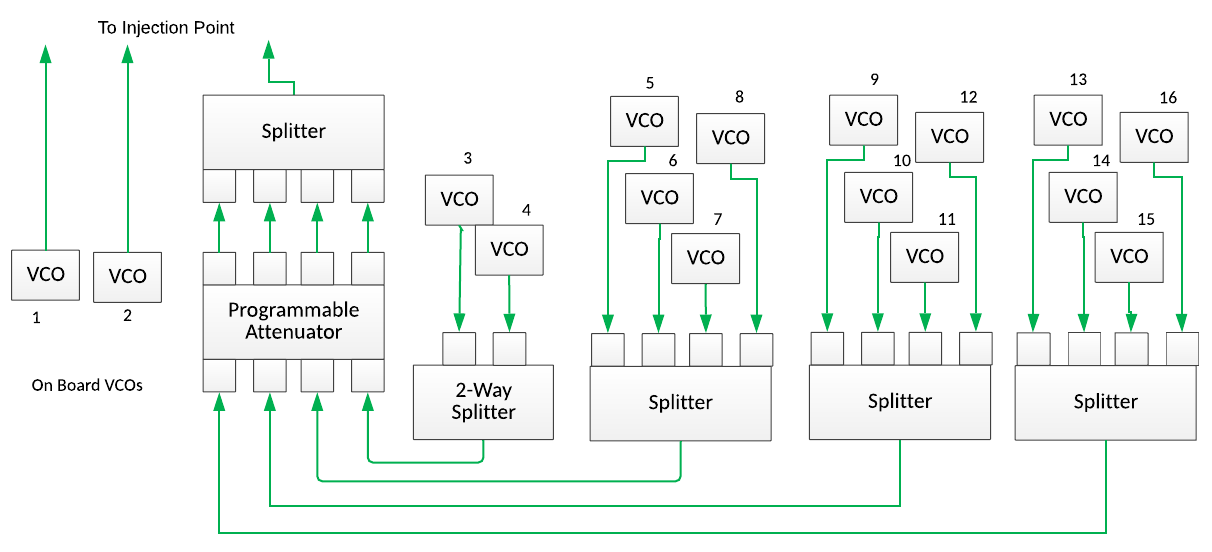
\includegraphics[width = 6 in]{Altimeter_Signal_Simulator.png}
\caption{Diagram of Combined 16 Simulated ALtimeter Signals}

\label{fig:VCO_Coupler}

\end{figure}
Each VCO was configured to simulate the RF power of an altimeter (typically 30~dBm), and the associated path loss from interferer TX to victim RX. This was accomplished with a variety of sources of attenuation. Each VCO output 4~dBm of RF power according to the data-sheet. Fixed attennuators could be placed at the RF output of each VCO to achieve individualized IPL values. Each splitter contributed 6~dB of attenuation to a connected path. The 4-channel programmable attenuator offered programmable values between 0 and 63~dB of attenuation. Lab measurements found that the programmable attenuator contributed 4~dB with a programmed setting of 0 and confirmed that each dB of programmed attenuation added one dB to this value. Finally, the attenuation from the interference injection point to the altimeter RX is added to the path loss. 

\begin{table}[]
\begin{tabular}{c||ccccc}
\textbf{VCO} & Power {[}dBm{]} & Fixed {[}dB{]} & Programmable {[}dB{]} & Path Loss {[}dB{]} & Power at RX {[}dBm\} \\ \hline
\textbf{1}   & 4               & -18              & X                     & -16                & -30                  \\
\textbf{2}   & 4               & -18              & X                     & -16                & -30                  \\ \hline


\textbf{3}   & 4               & 0              & -56                   & -40                & -92                  \\
\textbf{4}   & 4               & 0              & -56                   & -40                & -92                   \\ \hline


\textbf{5}   & 4               & 0              & -26                    & -40                & -62                 \\
\textbf{6}   & 4               & 0              & -26                    & -40 			& -62                  \\
\textbf{7}   & 4               & 0              & -26                    & -40                & -62                  \\
\textbf{8}   & 4               & 0             & -26                    & -40                & -62                  \\ \hline


\textbf{9}   & 4               & 0              & -26                   & -40                & -62                  \\
\textbf{10}  & 4               & 0              & -26                   & -40                & -62                  \\
\textbf{11}  & 4               & -23            & -26                   & -40               & -85                  \\
\textbf{12}  & 4               & -23             & -26                   & -40                & -85                  \\ \hline


\textbf{13}  & 4               & 0              & -49                   & -40                & -85                  \\
\textbf{14}  & 4               & 0              & -49                   & -40                & -85                  \\
\textbf{15}  & 4               & 0              & -49                   & -40                & -85                  \\
\textbf{16}  & 4               & 0              & -49                   & -40                & -85                 
\end{tabular}
\caption{VCO Attenuation Configurations for 200ft Worst Case}
\label{tab:VCO_Pow}
\end{table}
\subsubsection{Calibrating the VCOs}
The VCOs ordered for this purpose could go beyond the 4.2-4.4~GHz range, but a control voltage did not necessarily map to the same frequency across different VCOs. This meant that each of the 16 VCOs needed to be calibrated. First, each VCO was connected to a 5V power supply, and the control pin was connected to a separate power supply. The RF output of each VCO was connected to the spectrum analyzer for observation. The frequency output by a VCO under constant voltage had a bit of a `wobble' to it, so the spectrum analyzer was configured to display a \textit{Max Hold} instead of a real time measurement. After a VCO was left on a control voltage for several seconds, a marker was used to locate the frequency of the maximum output at that setting. 

The first calibration sweep went from 0 to 5~V in 1~V increments.  The goal of this broad sweep was to get an approximation for where the 4.2 and 4.4~GHz voltages were for each VCO. The VCO output was observed on the spectrum analyzer to determine the operating frequency at that control voltage. The search found that a majority of the 4.2--4.4~GHz band lied in the 2--5~V range for these VCOs. The initial sweep was not fine enough to capture the desired minimum and maximum frequencies for each VCO. 


% Please add the following required packages to your document preamble:
% \usepackage{booktabs}
\begin{table}[]
\centering
\begin{tabular}{@{}c|cc|cc|ccc@{}}
    & \multicolumn{2}{c|}{Lower} & \multicolumn{2}{c|}{Upper} & \multicolumn{3}{c}{\textbf{Function Generator Setting}}       \\
VCO & Voltage  & Freq {[}GHz{]}  & Voltage  & Freq {[}GHz{]}  & \textbf{Center} & \textbf{Amplitude} & \textbf{Freq {[}Hz{]}} \\ \midrule
1   & 2.2      & 4.237           & 4.0      & 4.362           & 3.1             & 1.8                & 143                    \\
2   & 1.6      & 4.236           & 3.5      & 4.367           & 2.6             & 1.9                & 143                    \\
3   & 2.2      & 4.232           & 4.1      & 4.365           & 3.2             & 1.9                & 143                    \\
4   & 2.0       & 4.233           & 3.9      & 4.364           & 3.0             & 1.9                & 111                    \\ \midrule
5   & 1.8      & 4.233           & 3.7      & 4.364           & 2.8             & 1.9                & 133                    \\
6   & 2.0      & 4.238           & 3.8      & 4.362           & 2.9             & 1.8                & 133                    \\
7   & 1.8      & 4.233           & 3.7      & 4.365           & 2.8             & 1.9                & 133                    \\
8   & 1.7      & 4.233           & 3.6      & 4.368           & 2.7             & 1.9                & 118                    \\ \midrule
9   & 2.0      & 4.235           & 3.9      & 4.367           & 3.0             & 1.9                & 118                    \\
10  & 2.0      & 4.233           & 3.9      & 4.365           & 3.0             & 1.9                & 118                    \\
11  & 2.0      & 4.238           & 3.8      & 4.362           & 2.9             & 1.8                & 111                    \\
12  & 2.1      & 4.236           & 3.8      & 4.366           & 3.0             & 1.7                & 129                    \\ \midrule
13  & 1.8      & 4.235           & 3.7      & 4.364           & 2.8             & 1.9                & 129                    \\
14  & 2.0      & 4.235           & 3.7      & 4.366           & 2.9             & 1.7                & 129                    \\
15  & 2.1      & 4.237           & 3.8      & 4.368           & 3.0             & 1.7                & 143                    \\
16  & 2.3      & 4.233           & 4.2      & 4.365           & 3.3             & 1.9                & 143                   
\end{tabular}
\caption{VCO Calibration Results and Corresponding Function Generator Settings}
\label{tab:VCO_Cal}
\end{table}


A second calibration was attempted to fix this. The goal was to get the simulated FMCW waveforms centered at 4.3 GHz, with a span of $\pm65$~MHz. Using 100~mV increments, the previous calibration procedure was repeated, this time explicitly searching for the control voltages corresponding to the frequencies closest to 4235~MHz and 4365~MHz. These were achieved with a $\pm3$~MHz precision. The 100~mV increments from the calibration process were chosen due to the precision available to the function generators. It was this limitation that lead to the 3~MHz frequency precision. The full calibration results are shown in Table~\ref{tab:VCO_Cal}.

Once the lower and upper voltages were determined, a simple calculation found the center voltage and amplitude necessary to feed into the function generators. In addition to the amplitude and offset settings available to the function generator, the control voltage wave had a frequency parameter. These were chosen in part with enough variance so that there was no synchronization between the different simulated altimeter signals. Random crossover of the simulated altimeter signals was desired to closely match the real world interference scenario. Function generator parameters are also shown in Table~\ref{tab:VCO_Cal}.

\subsubsection{VCO Protection Circuit}
While the VCO's were designed to operate with a control voltage between 0 and 5~V, they were later verified to tolerate a maximum 6.5~V signal before a catastrophic failure. Because the Function Generators were capable of up to a 20~V peak to peak signal, they could damage a VCO with an accidental twist of a knob, and a protection circuit was needed.

\begin{figure}[ht]
\centering
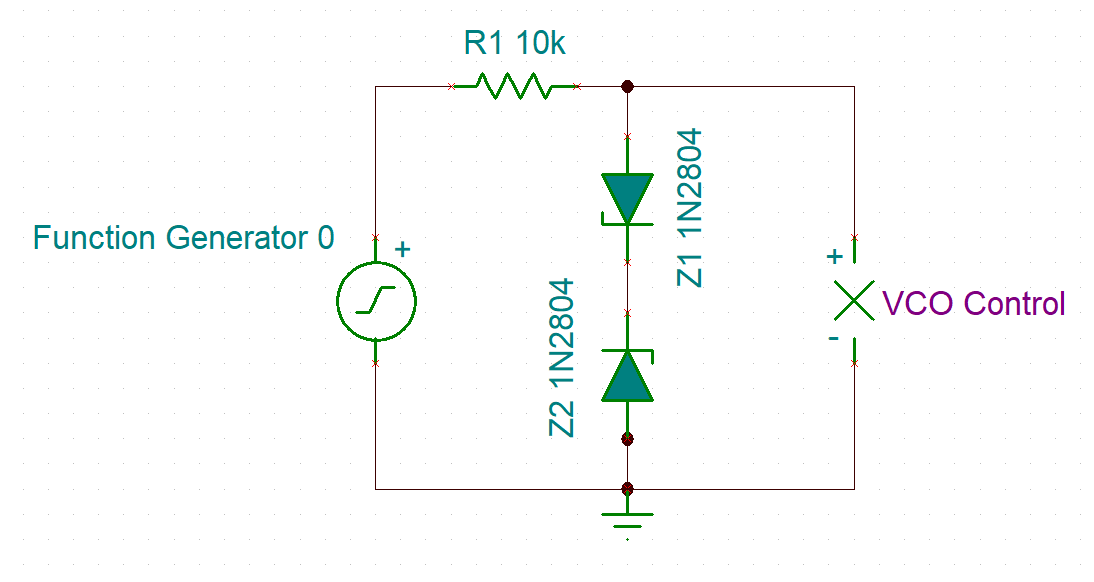
\includegraphics[scale=.6]{Protective_Circuit.png}
\caption{Double Clipper Protective Circuit}

\label{fig:Clipper}

\end{figure}


 Initially, the protective circuit seemed even more urgent. The voltage setting on the function generator starts at 10~V upon power up, but does not clearly mark whether this is a peak to peak voltage or $\pm10$~V. Compounding this ambiguity, when the output of the function generators was measured with an oscilloscope, the multiplier setting was set to 2X. This made it appear to be a $\pm10$~V signal on startup which would fry the VCO if the function generator was accidentally power cycled. This error was only noticed after the protective circuit was designed and built. 

After some searching, a limiter or `clipper' circuit was decided on to protect the VCOs. Clippers consist of a resistor and one or two diodes. Various designs of clipper circuits and the trade-offs between them are discussed in~\cite{sedra_microelectronic_2015}. Based on this discussion, a double clipper like the one shown in Figure~\ref{fig:Clipper} was decided on. Two Zener diodes begin to limit the upper and lower voltage extremes once they pass the diode's cutoff voltage. A resistor is placed in series with the diodes to limit the current in the diodes to safe levels. 
\begin{figure}[ht]
\centering
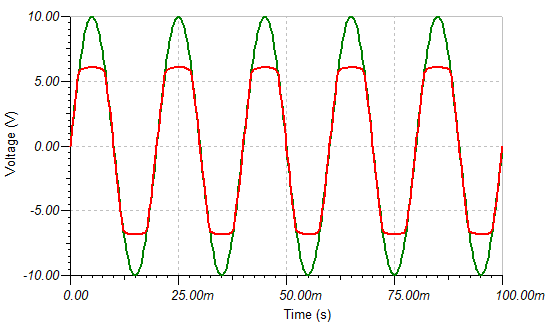
\includegraphics[scale=1.3]{Clipped_Sin_Wave.png}
\caption{Double Clipper Protective Circuit}

\label{fig:Clipped_Sin}

\end{figure}

The clipper circuit was modeled in a spice program so that different diode cutoff voltages could be tried. Simulations showed that the output voltage from this circuit would typically go slightly above the cutoff voltage. Because of this, a Zener diode with a 6~V cutoff was chosen to limit the output below the 6.5~V failure point. A simulated ouptut from the clipper circuit waveform is shown in Figure~\ref{fig:Clipped_Sin}. A $\pm$10~V sine wave is fed from the function generator, shown in green, and the `clipped' waveform is shown in red. The circuit allows voltages close to the failure point without reaching it. This performance was verified with an oscilloscope for each function generator output.


\subsection{Testing Lower Altitudes}
A final major modification from the initial test regimen involved adding different altitude simulator configurations to the rotation to achieve lower altitudes. These were touched on briefly in Section~\ref{sub:Implementing}. Lower altitude tests were first started before the approach scenario analysis determined that 200~ft was the worst case scenario. Once the worst case analysis was determined, lower altitude tests were continued to provide supplementary evidence at another altitude in the landing scenario. 
\begin{figure}[ht]
\centering
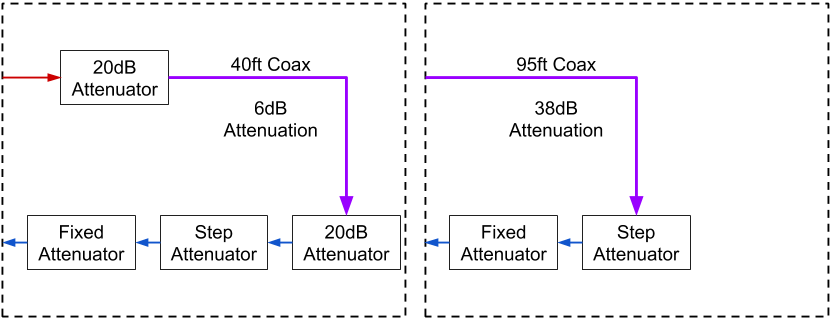
\includegraphics[width = 6 in]{Low_Altitude_Simulator.png}
\caption{Left: 40ft Altitude Simulator; Right: 95 ft Altitude Simulator}

\label{fig:Low_Altitudes}

\end{figure}

Two different coaxial cables were used to simulate different altutudes below the 500~ft threshold the optical delay line was capable of. Firstly, a coaxial cable providing 40~ft altitude was located in the lab for this purpose, shown on the left of Figure~\ref{fig:Low_Altitudes}. When measured with a VNA, this coax had only a 6~dB attenuation, so two 20~dB fixed attenuators were placed on either side to increase the attenuation. This allowed the same step and fixed attenuator combination from Figure~\ref{fig:Altitude_Simulator} to easily achieve the DO-155 attenuation from Table~\ref{tab:loop loss}. The 40~ft altitude simulator underwent the same modification as the Fiber Optic Line in Figure~\ref{fig:coupler_swap}, which allowed higher power interference signals without modifying the fixed and step attenuator settings in use. 

The second altitude simulator used during these tests was a 95~ft cable which was ordered after a significant nubmer of 40~ft tests had been run. The 40~ft tests had revealed a problem where one of the newer altimeters (with more advanced signal processing) would not output an altitude below a certain threshold unless it detected that the aircraft was moving. This precipitated the 95~ft tests so that an altitude below the 200~ft worst case could be tested across all units. The 95ft cable was a lower quality coax than the 40~ft cable, and when measured with a network analyzer showed an approximately 38~dB attenuation at 4.3~GHz. This was confirmed to be approximately the expected attenuation for this length of coax from the manufacturer's website. Once again, a fixed and step attenuator allowed the altitude simulator to be fully adjustable and achieve the DO-155 specified attenuation. 

%%%%%%%%%%%%%%%%%%%%%%%%%%%%%%%%%%%%%%%%%%%%%%%%%%%%%%%%%
\section{Expanded Setup Test Plans}
The different modifications discussed above were combined into a full setup. This was used to test the altimeters in approach scenarios, to detremine a breaking point for full spectrum interference for the purposes of regulation, and to investigate the effects of adjacent band interference signals.
\subsection{Full Setup Diagram}
\begin{figure}[ht]
\centering
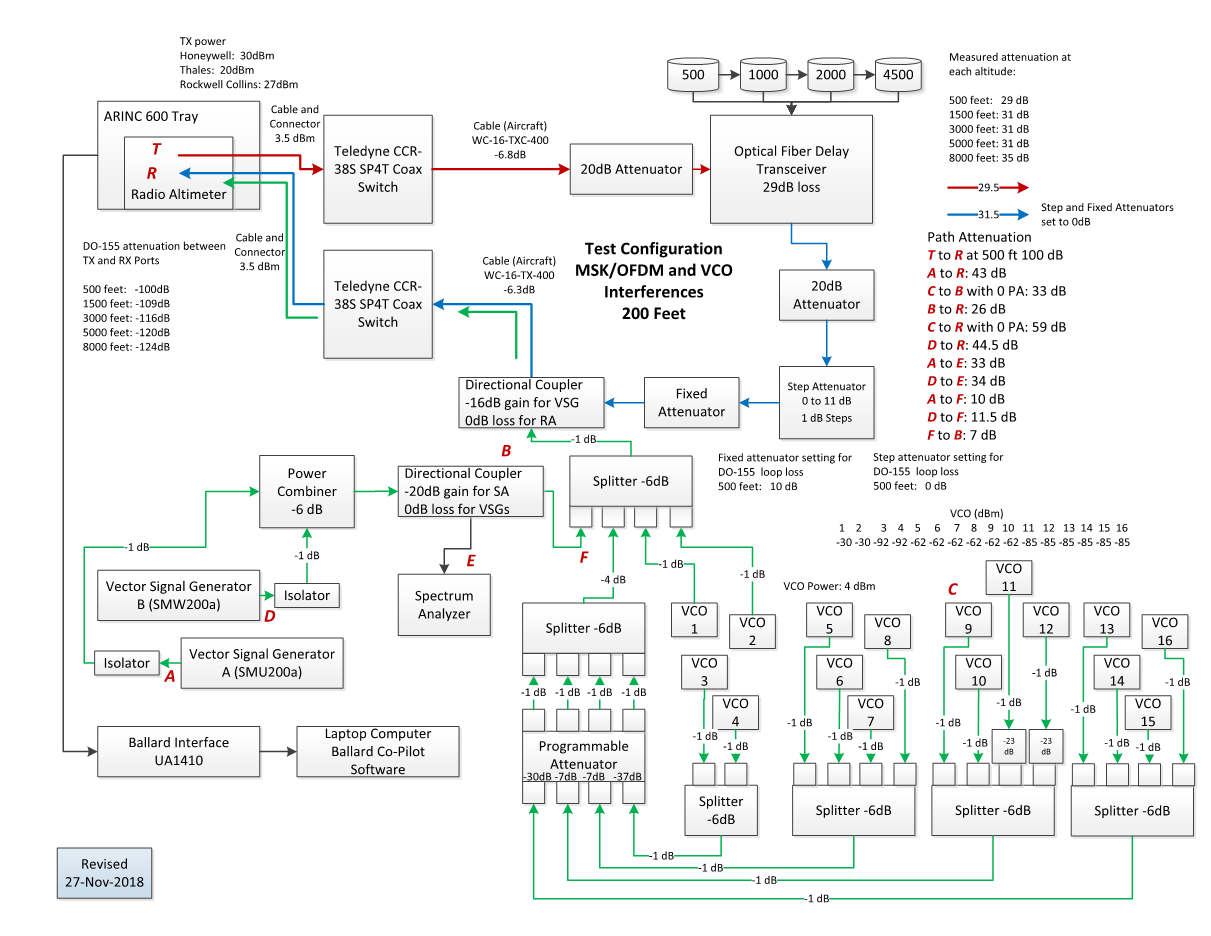
\includegraphics[width = 6 in]{Full_Setup.PNG}
\caption{Full test setup combining various modifications to Figure~
\ref{fig:Initial}}

\label{fig:combined}

\end{figure}
Figure~\ref{fig:combined} shows the full test setup diagram. The modifications covered in Section~\ref{sec:expanding}, including the second VSG, isolators to protect the VSG's, and the VCO setup to simulate 16 other altimeter signals are included in this diagram. Depending on the desired test scenario, the lower altitude simulators from Figure~\ref{fig:Low_Altitudes} were substituted in for the optical delay line, and as tests progressed, the modification shown in Figure~\ref{fig:coupler_swap} allowed for higher interference powers. 

\subsection{Breaking Point Definition}\label{sub:break}
Early tests showed that powerful itnerference signals would not only cause outliers which broke the ARINC 707~\cite{noauthor_arinc_2009} standards, but also caused a distortion of the mean height. Since presenting a more restrictive standard to regulators was seen as beneficial, a stronger definition of breaking point was introduced compared to previous tests. Thus, the breaking point definition was expanded to include either (i) a maximum height error beyond the 2\% or 1.5~ft allowable by ARINC 707, (ii) any height reading labeled NCD, or (iii) a mean height error greater than 0.5\%. 

\subsection{In Band Testing}\label{sub:ib}
\begin{table}[]
\begin{tabular}{c|c|c|c|c|c|c|c}
\multicolumn{3}{c|}{\textbf{Interference Signal}} & \multicolumn{3}{c|}{\textbf{VSG RF Power}} & \multicolumn{2}{c}{\textbf{Power Durations}} \\
Modulation    & Bandwidth   & Center     & Min         & Step    & Max       & ON                & OFF              \\ \hline
OFDM          & 200 MHz     & 4300 MHz   & -56 dBm     & 2 dB    & 19 dBm    & 60 s              & 20 s            
\end{tabular}
\caption{Interference Signals for Wideband Testing}
\label{tab:Wideband}
\end{table}


Table~\ref{tab:Wideband} shows the interference signals used to run the in band dual vsg tests. The purpose of these tests was to find the `breaking point' of each altimeter when subjected to a full band of interference signals under worse than possible real life conditions. When the worst breaking point among the altimeters sampled was found, the committee would add a margin of a few dB and propose that number to regulators. These results are discussed in Section~\ref{sec:dvsg_ib_results}

\subsection{Out of Band Testing}\label{sub:oob}
Finally, Table~\ref{tab:oob} shows a representative test definition for the out of band tests run under AFE76s2. These tests were designed to develop an RF power mask on the upper and lower side of the radio altimeter bands. This mask could be brought to regulators with a proposal to limit users in adjacent bands a certain margin below the altimeter breaking point. 

Initially, the 5~MHz wide OFDM signals used in previous tests were tried. However, after initial results came in, more granular sweep was desired, so the bandwidth was reduced to the 200~kHz signals shown in Table~\ref{tab:oob}. When the 200~kHz waveform was measured on the spectrum analyzer, it was noticed that the waveform center was slightly offset from the carrier frequency. The lower edge of the waveform was approximately 35~kHz below the carrier, and the upper edge was approximately 165~kHz above the carrier. 

Since the test goal was to step an OFDM waveform with the upper edge directly on 4.2~GHz, and step away from the altimeter band till the upper edge was 5~MHz away from the band edge. Waveforms in the upper adjacent band were placed at 4200.035~MHz and stepped to 4205.035~MHz for the same reason.

These tests are ongoing at the time of writing, and will likely go through a few more iterations before being finalized, but preliminary results from this test definition are discussed in Section~\ref{sec:dvsg_oob_results}.

\begin{table}[]
\begin{tabular}{cc|cc|ccc|cc}
\multicolumn{4}{c|}{\textbf{Interference Signal}}                                     & \multicolumn{3}{c|}{\textbf{VSG RF Power}} & \multicolumn{2}{c}{\textbf{Durations}} \\
                                &           & \multicolumn{2}{c|}{Center Frequencies} &                &            &              &                               &         \\
\multicolumn{1}{c|}{Modulation} & Bandwidth & Min {[}MHz{]}      & Max {[}MHz{]}      & Min            & Step       & Max          & \multicolumn{1}{c|}{ON}       & OFF     \\ \hline
\multicolumn{1}{c|}{OFDM}       & 200 kHz   & 3900           & 4200         & -14 dBm        & 2 dB       & 18 dBm       & \multicolumn{1}{c|}{10 s}     & 5 s    \\
\multicolumn{1}{c|}{OFDM}       & 200 kHz   & 4400      & 4700 & -14 dBm        & 2 dB       & 18 dBm       & \multicolumn{1}{c|}{10 s}     & 5 s   
\end{tabular}
\caption{Interference Signals For Out Of Band Testing}
\label{tab:oob}
\end{table}
